\documentclass[master=eelt,masteroption=ec]{kulemt}
\setup{% Remove the "%" on the next line when using UTF-8 character encoding
  inputenc=utf8,
  title={The best master's thesis ever},
  author={First Author\and Second Author},
  promotor={Prof.\,dr.\,ir.\ Knows Better},
  assessor={Ir.\,Kn. Owsmuch\and K. Nowsrest},
  assistant={Ir.\ An~Assistent \and A.~Friend}}
% Remove the "%" on the next line for generating the cover page
%\setup{coverpageonly}
% Remove the "%" before the next "\setup" to generate only the first pages
% (e.g., if you are a Word user).
%\setup{frontpagesonly}

% Choose the main text font (e.g., Latin Modern)
\setup{font=lm}

% If you want to include other LaTeX packages, do it here. 

% Finally the hyperref package is used for pdf files.
% This can be commented out for printed versions.

\usepackage[pdfusetitle,colorlinks,plainpages=false]{hyperref}

%%%%%%%
% The lipsum package is used to generate random text.
% You never need this in a real master's thesis text!
\IfFileExists{lipsum.sty}%
 {\usepackage{lipsum}}%
 {\newcommand{\lipsum}[1][1-7]{\par And some text: lipsum ##1.\par}}
%%%%%%%

%\includeonly{chap-n}
\begin{document}

\begin{preface}
    I would like to thank everybody who kept me busy the last year,
    especially my promoter and my assistants. I would also like to thank the
    jury for reading the text. My sincere gratitude also goes to my wive and
    the rest of my family. \cite{aires-2020-information}
\end{preface}

\tableofcontents*

\begin{abstract}
    In today's digital, information-rich society, \textbf{media} bias poses a significant challenge to the objectivity and credibility of news reporting. As someone living in our current society, one has inevitably encountered some form of bias in the media, either consciously or unconsciously. Media bias can shape our perceptions, influence our opinions, and affect our understanding on various issues. It is crucial to recognise and address this bias to ensure a well-informed and balanced perspective. By being aware of the inherent biases in media sources, individuals can critically evaluate the information they consume and seek out diverse viewpoints to form a more comprehensive understanding of the world.
    In this paper...
\end{abstract}

% A list of figures and tables is optional
%\listoffigures
%\listoftables
% If you only have a few figures and tables you can use the following instead
\listoffiguresandtables
% The list of symbols is also optional.
% This list must be created manually, e.g., as follows:
\chapter{List of Abbreviations and Symbols}
\section*{Abbreviations}
\begin{flushleft}
    \renewcommand{\arraystretch}{1.1}
    \begin{tabularx}{\textwidth}{@{}p{12mm}X@{}}
        LoG  & Laplacian-of-Gaussian      \\
        MSE  & Mean Square error          \\
        PSNR & Peak Signal-to-Noise ratio \\
    \end{tabularx}
\end{flushleft}
\section*{Symbols}
\begin{flushleft}
    \renewcommand{\arraystretch}{1.1}
    \begin{tabularx}{\textwidth}{@{}p{12mm}X@{}}
        42    & ``The Answer to the Ultimate Question of Life, the Universe,
        and Everything'' according to \cite{h2g2}                            \\
        $c$   & Speed of light                                               \\
        $E$   & Energy                                                       \\
        $m$   & Mass                                                         \\
        $\pi$ & The number pi                                                \\
    \end{tabularx}
\end{flushleft}

% Now comes the main text
\mainmatter

\chapter{Introduction}
\label{cha:1}

This thesis project is part of an Advanced Master of Artificial Intelligence programme—Speech and Language Technology, conducted in collaboration with the Media Bias Group \cite{media-bias-group}, who provided the topic and additional guidance along the project. The introduction chapter provides a general overview of the project, outlining its motivations, goals, and contributions.


\section{Motivation}

Media bias is widespread in today's landscape, particularly on matters such as health, climate, and politics \cite{suarez-2021-prevalence-health-misinformation,wang-2024-health-misinformation,fleming-2023-climate-disinformation,tiedemann-2024-misinformation-democracy}. The existence of media bias in news sources can and has been used as a way to shape and influence public opinion \cite{aires-2020-information}. The advent of social media has exacerbated the spread of misinformation, allowing false information to easily and rapidly circulate while remain unchecked \cite{froehlich-2024-misinformation}. A survey by \cite{allcott-2017-fake-news-election} indicated that fake news on social media played a significant role in the election of President Trump in 2016. During the COVID-19 pandemic, numerous conspiracy theories gained widespread traction through the media, with substantial support from large groups of people. A 2020 Harvard survey revealed that nearly 20\% of people believed the pandemic was a ploy "to install tracking devices inside our bodies" \cite{enders-2020-covid19-misinformation}. Despite being a major societal issue, research on the spread of misinformation on social media platforms remains scarce \cite{muhammed-2022-disaster-of-misinformation}.

\begin{figure}[htbp]
    \centering
    \fbox{
        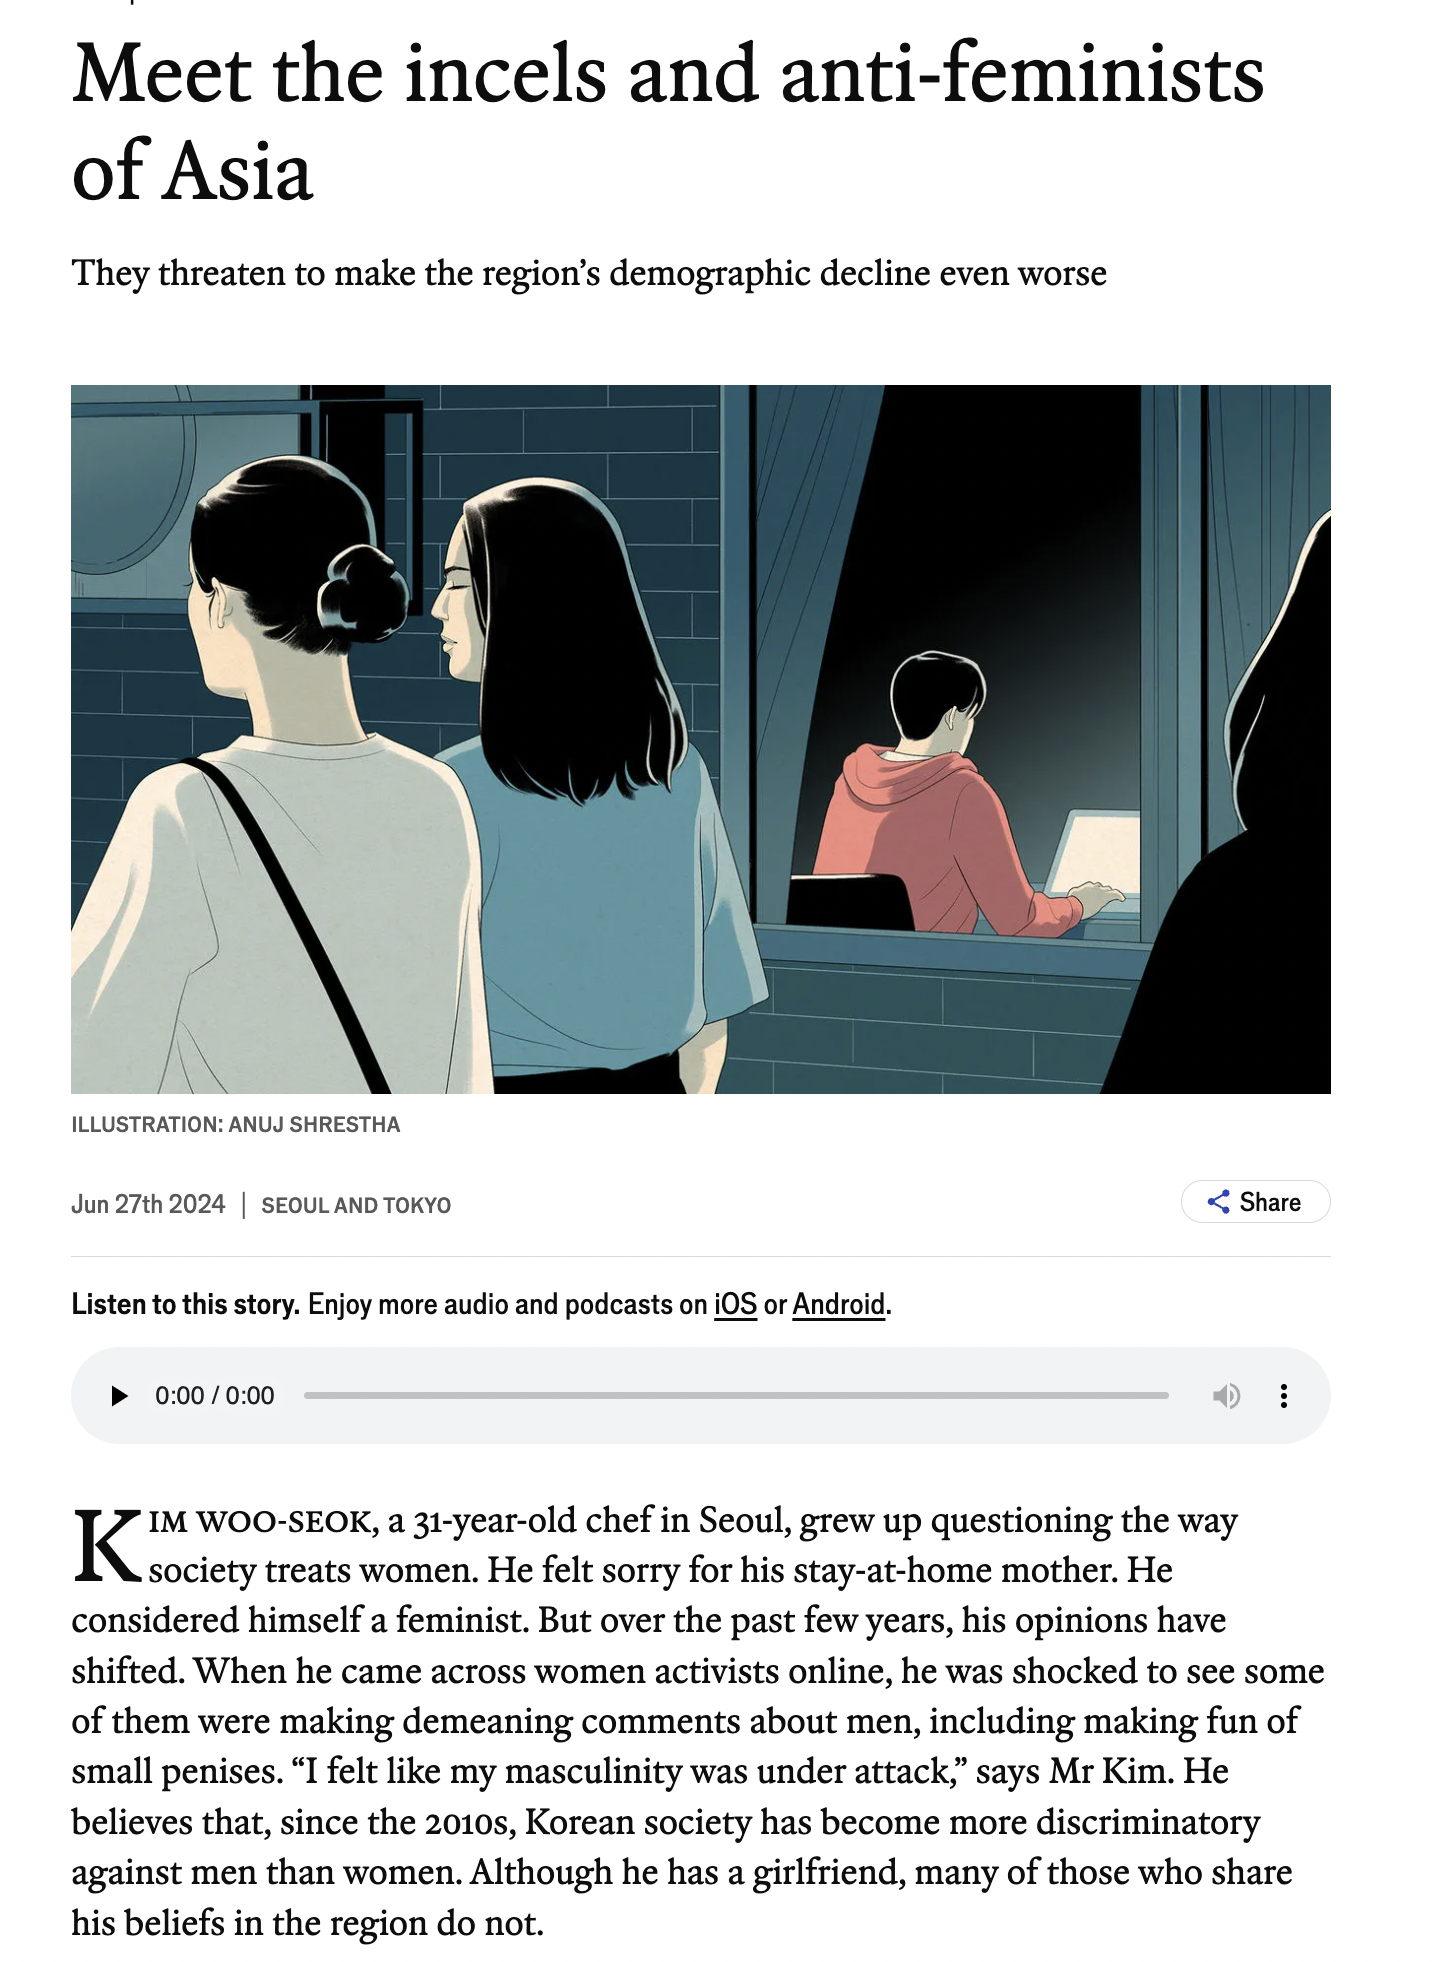
\includegraphics[width=0.6\linewidth]{images/the-economist-biased-article.png}}
    \caption{A recent article from The Economist \cite{economist-2024-incels} portraying gender discrimination with a negatively framed headline}
    \label{fig:the-economist-biased-article}
\end{figure}

An example of a biased article can be seen in a recent piece published by The Economist \cite{economist-2024-incels}, shown in Figure \ref{fig:the-economist-biased-article}. The author presents the information in a way that could be considered biased due to its choice of language, implied causation, and lack of context. Published in June 2024, this example proves that media bias exists and is prevalent even in prominent news outlets like The Economist.

Ideally, unbiased media content that objectively and fairly represents multiple or a range of perspectives is desirable, news sources should remain neutral and let readers build their own opinions on the subject \cite{reuters-2021-digital-news-report}. However, this is often unachievable due to human capabilities and resource limitations; journalists cannot possibly possess complete knowledge on every topic, be physically present everywhere, or interview every relevant individual on a significant subject \cite{allsides-2022-bias-definition}. Truth and journalism objectivity is a complex matter full of choices and dilemmas, where ultimately it falls on the journalists' own preferences and criteria \cite{boudana-2011-journalistic-objectivity}. A survey found evidence that journalists' personal beliefs substantially influence their news decisions, expressed within the stories they choose and the statements they write \cite{patterson-donsbach-1996-news-decisions}.

Therefore, instead of eliminating media bias, our goal should be to draw attention to its existence and forms, giving readers awareness of such content \cite{spinde-2024-taxonomy}, ultimately building a tool to defend readers from media manipulation, political agenda or indoctrination. This is essential to ensure that readers are able to form their own choices and opinions with utmost honesty and transparency.

% Journalism has abandoned the idea of seeking neutrality and objectivity, aiming instead to adopt a more engaged and committed approach. Objectivity in the media has been rejected both as an impossible standard and as an undesirable norm. \cite{boudana-2011-journalistic-objectivity}.

While there exist organisations consisting of expert annotators that manually read and review articles \cite{adfontes, allsides, mbfc}, there is a growing need for more efficient methods of media bias detection. Automatic media bias detection offers a promising alternative, as developing robust systems could enhance scalability and consistency in identifying biases across a vast array of articles, addressing the limitations of manual review processes. However, this field remains relatively new, under-resourced, and challenging, due to the lack of a universally accepted definition of bias and its subtlety, which can make it difficult to identify \cite{rodrigo-2024-systematic-review-media-bias}.

Available media bias datasets \cite{spinde-2021-babe,fan-2019-basil,chen-2020-nlpcss,spinde-2023-bat,gruppi-2023-nela-gt-2022} are either limited in size or contain low-level, ambiguous annotations. In addition, these datasets vary in format, cover different sets of topics, contain different types of bias, and, more importantly, use different labelling formats, making it particularly difficult to compare and evaluate different media bias datasets and models trained on them. There is a critical need to develop new, richer datasets that are more extensive and varied, preferably covering a broader array of events and domains \cite{rodrigo-2024-systematic-review-media-bias}.

Existing works in media bias classification tend to have major drawbacks \cite{maab-2023-lexical-bias-detection, maab-2023-target-aware, guo-2022-modeling, van-den-berg-2020-context,lee-2021-unifying,lei-2022-sentence,lei-2024-event-relation}. The classification is mostly done on the sentence-level with binary output, which is far too naive and may miss the broader context and impact conveyed by an entire article. Sentence-level classifiers tend to also rely on low-level lexical information, which is proven to fail at the article-level \cite{chen-2020-detecting-media-bias-gaussian}. Moreover, different sentences within the same article can exhibit contradictory or varying biases \cite{lei-2022-sentence}. Thus, sentence-level classifiers are inadequate for accurately classifying media bias across an entire article. Since media content is typically presented as articles composed of numerous sentences, an effective article-level media bias classifier is both necessary and crucial.

While there are many studies focused on article-level political bias or ideology detection \cite{kulkarni-2018-multi-view,baly-2020-we-can-detect-your-bias,baly-2019-mt}, to my knowledge, there has been very little significant work on article-level media bias classification.

\section{Goals and Contributions}

The primary goal of this project is to develop a novel approach for article-level media bias classification, by considering State-of-the-Art (SOTA) transformer-based approaches, as well as techniques that have been proven to be successful in document classification \cite{su-2021-classifying,wan-2019-long-length,park-2022-efficient,pappagari-2019-hierarchical}. To achieve this, the project will address the following research questions:
\begin{enumerate}
    \item What are the challenges and limitations of article-level bias classification, and how can they be mitigated?
    \item How can current media bias datasets be improved to better support article-level classification?
    \item What are the most effective methods to represent articles and preserve contextual information for media bias classification task?
    \item How can an effective article-level media bias classifier be trained and evaluated?
\end{enumerate}

This thesis project makes three main contributions: (1) it investigates the current state of article-level media bias classification, identifying gaps in research and key challenges; (2) it reconstructs the BAT dataset by crawling articles content, resulting in a dataset of 5,497 articles with an additional multi-class labels; and (3) it examines various natural language processing (NLP) techniques for article-level media bias classification, highlighting that hierarchical methods show significant promise, slightly outperforming fine-tuning Longformer.

\section{About the Media Bias Group}

The Media Bias Group \cite{media-bias-group} was established in mid-2020 by Timo Spinde during his pursuit of a Ph.D. in computer science, having been integrated into the topic since his undergraduate studies, with a vision to aid others perceive news in a more balanced and conscious manner. After a year of planning how a system could uncover bias on a vast scale encompassing millions of articles, he founded the group and forged connections with various partners, particularly those relevant to specific aspects of the project. In just one year, the project has garnered support from multiple other research groups, with around twenty students from seven countries joining to contribute to the system.

The group is composed of a collective of scholars across various fields such as Psychology, Linguistics, and Computer Science, with a shared goal to comprehend the factors influencing human perception of news content as biased or one-sided. Currently, the network includes six main researchers and coordinators, twenty-one professors and postdocs, as well as eight active students. Numerous publications related to media bias have been published through the network into major conferences such as EMNLP 2021 \cite{spinde-2021-babe}.


%%% Local Variables: 
%%% mode: latex
%%% TeX-master: "thesis"
%%% End: 
\chapter{Background Information and Literature Review}
\label{cha:2}

This chapter provides background information on media bias, introduces general machine learning concepts, and covers relevant Natural Language Processing (NLP) techniques. Additionally, it related works on document classification and media bias classification are reviewed.


\section{Media Bias}

Allsides \cite{allsides-2022-bias-definition} defines media bias as "The tendency of news media to report in a way that reinforces a viewpoint, world-view, preference, political ideology, corporate or financial interests, moral framework, or policy inclination, instead of reporting in an objective way (simply describing the facts)". Media bias has existed and been researched since the 1950s \cite{white-1950-case-study-selection-news}.

\begin{figure}[htbp]
    \centering
    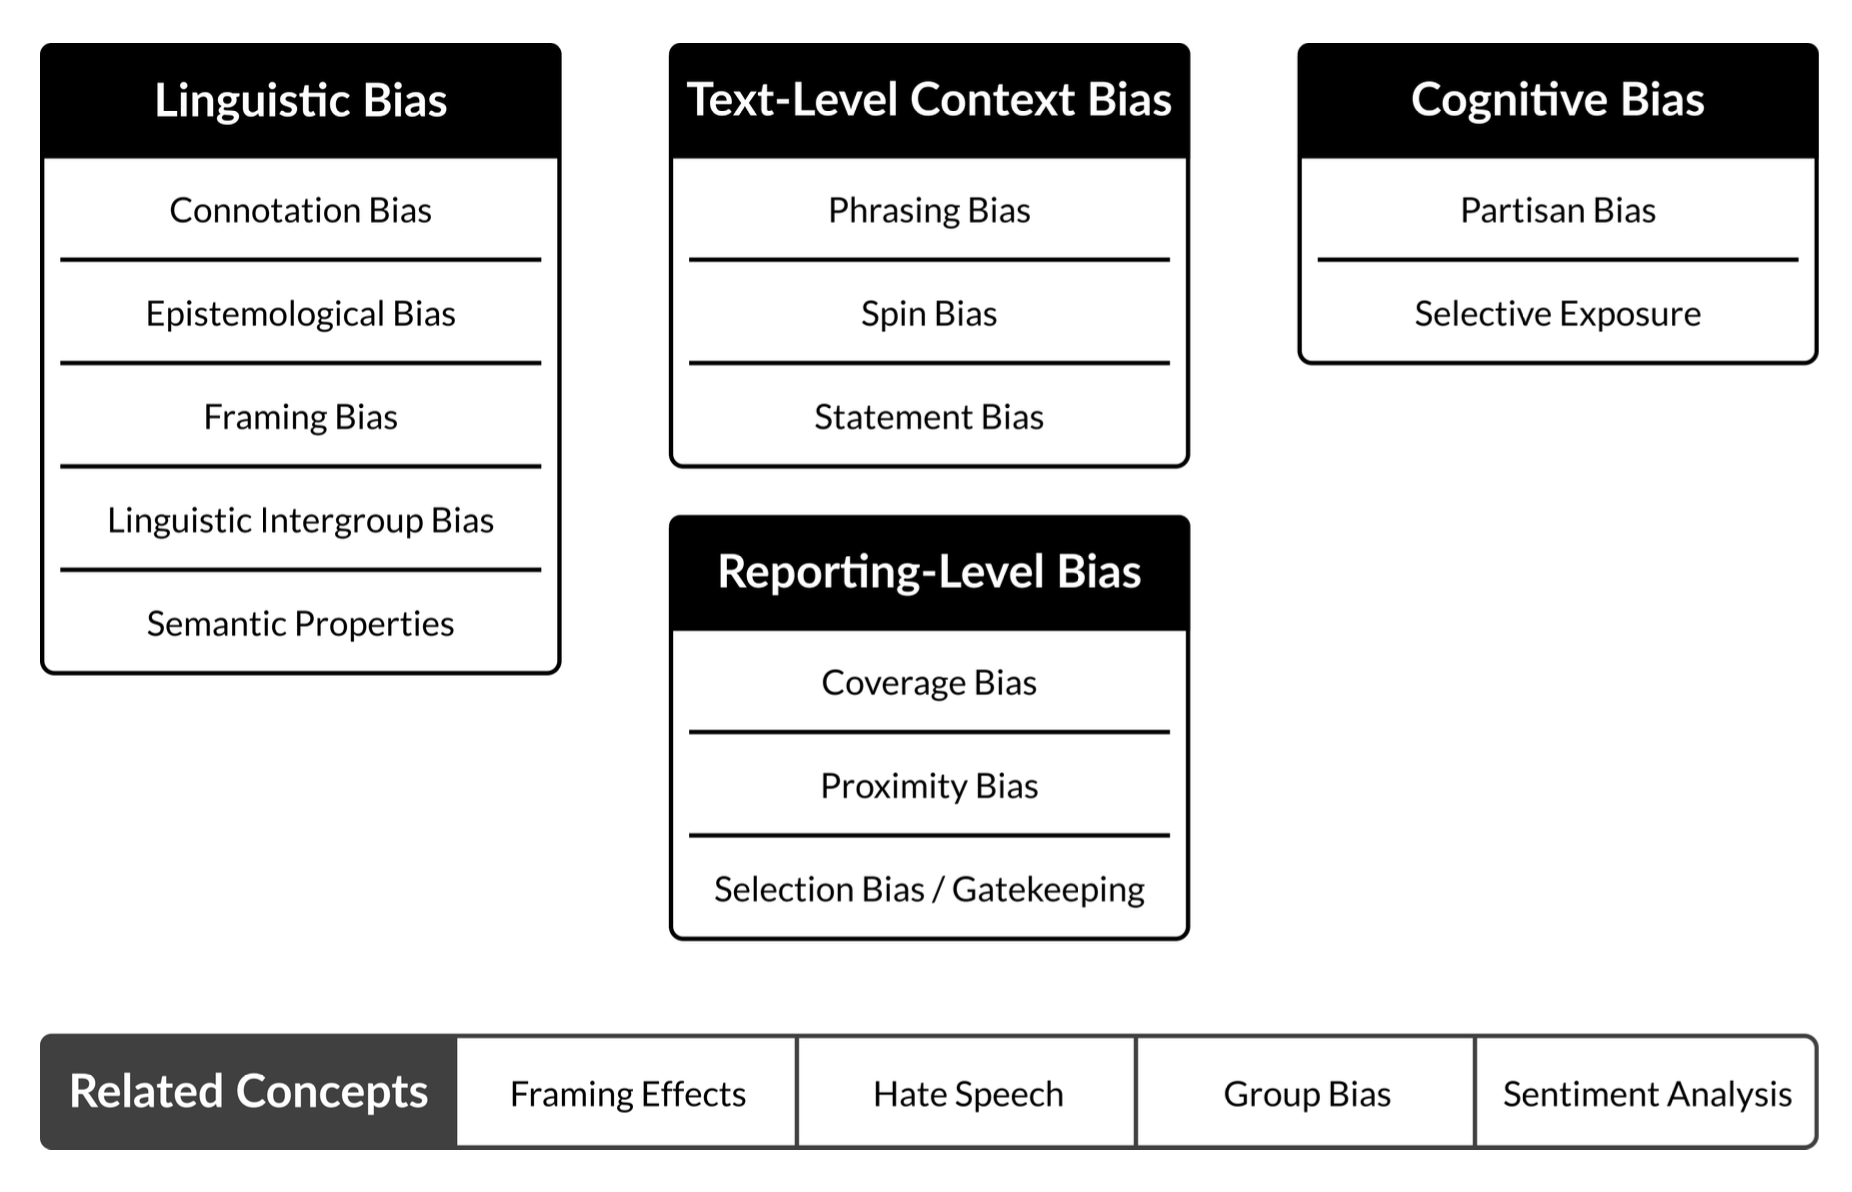
\includegraphics[width=0.9\linewidth]{images/bias-types-taxonomy.png}
    \caption{Media bias types as defined in The Media Bias Taxonomy \cite{spinde-2024-taxonomy}}
    \label{fig:media-bias-taxonomy}
\end{figure}

Many works and authors have tried to categorise media bias based on its types and characteristics \cite{rodrigo-2024-systematic-review-media-bias,eberl-2017-bias-political,spinde-2024-taxonomy,allsides-media-bias-types}. This project will follow The Media Bias Taxonomy by Spinde et al. (Figure \ref{fig:media-bias-taxonomy}), primarily focusing on \textbf{Text-level Context Bias}, which pertains to the context of a text and the manner in which it is conveyed \cite{spinde-2024-taxonomy}.

\begin{figure}[htbp]
    \centering
    \fbox{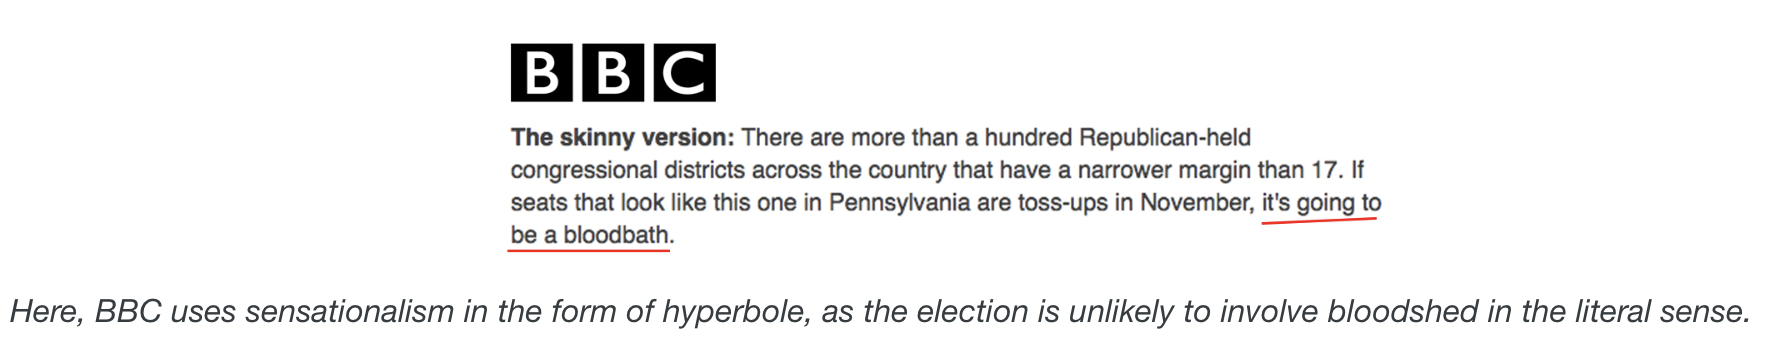
\includegraphics[width=0.95\linewidth]{images/phrasing_bias_example.png}}
    \fbox{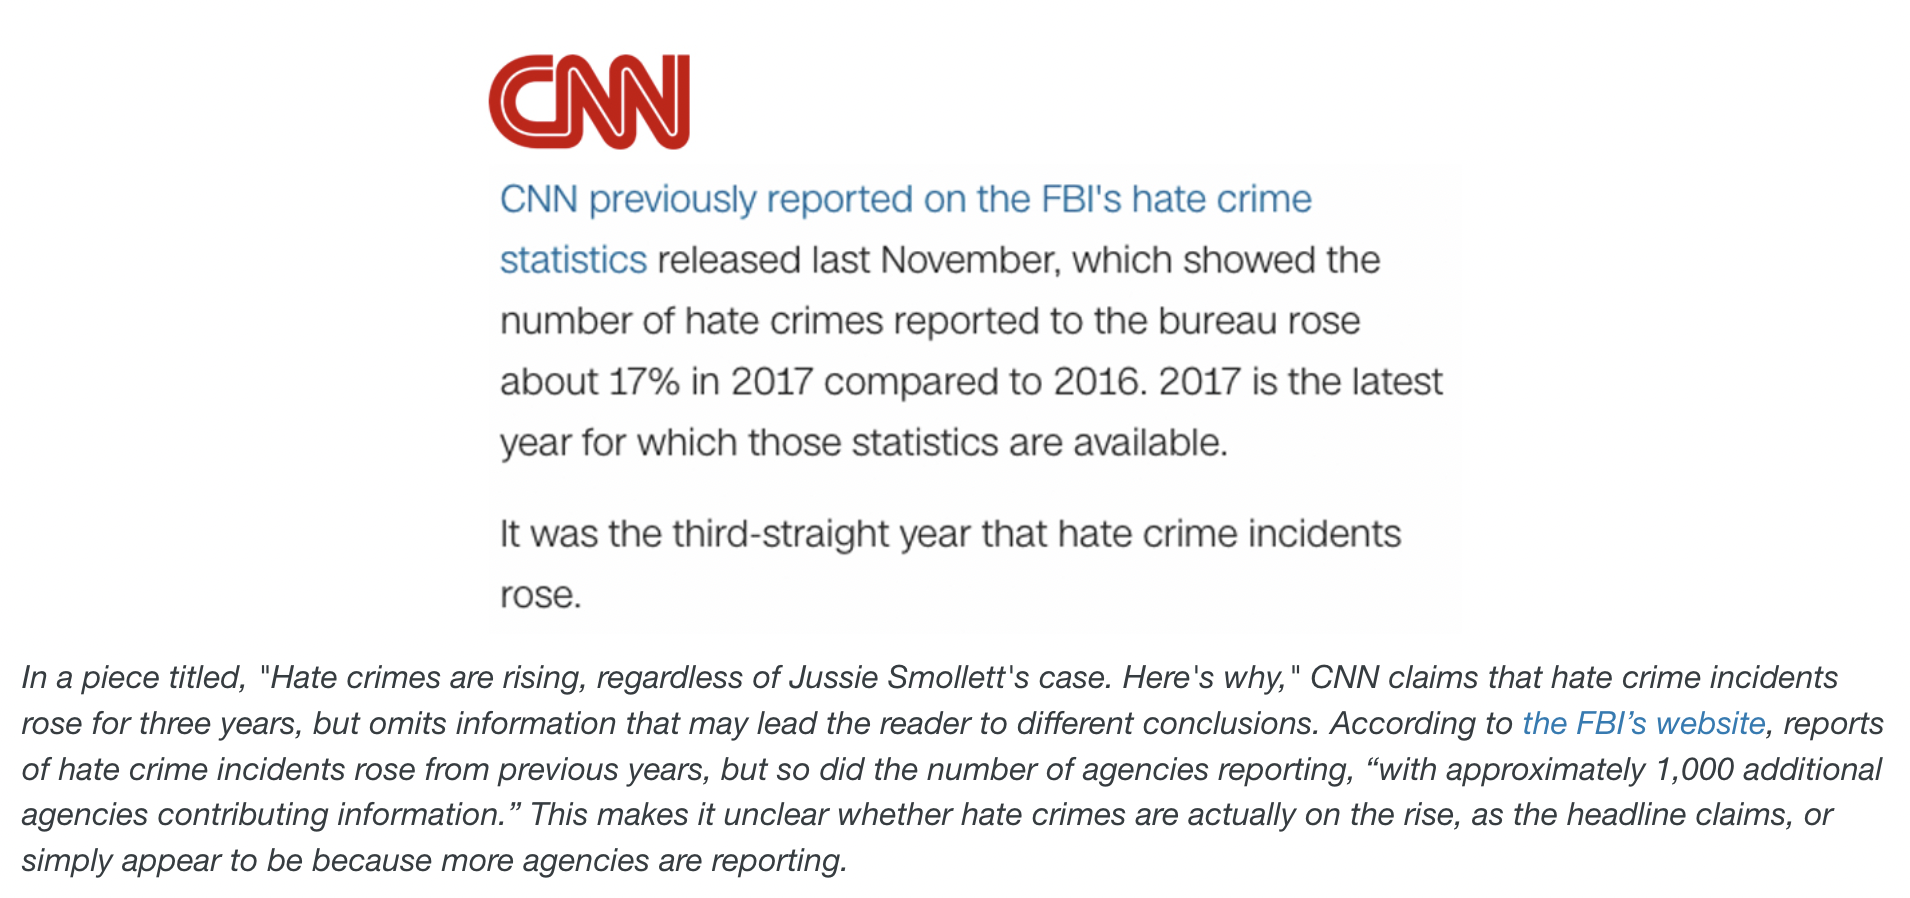
\includegraphics[width=0.95\linewidth]{images/spin_bias_example.png}}
    \fbox{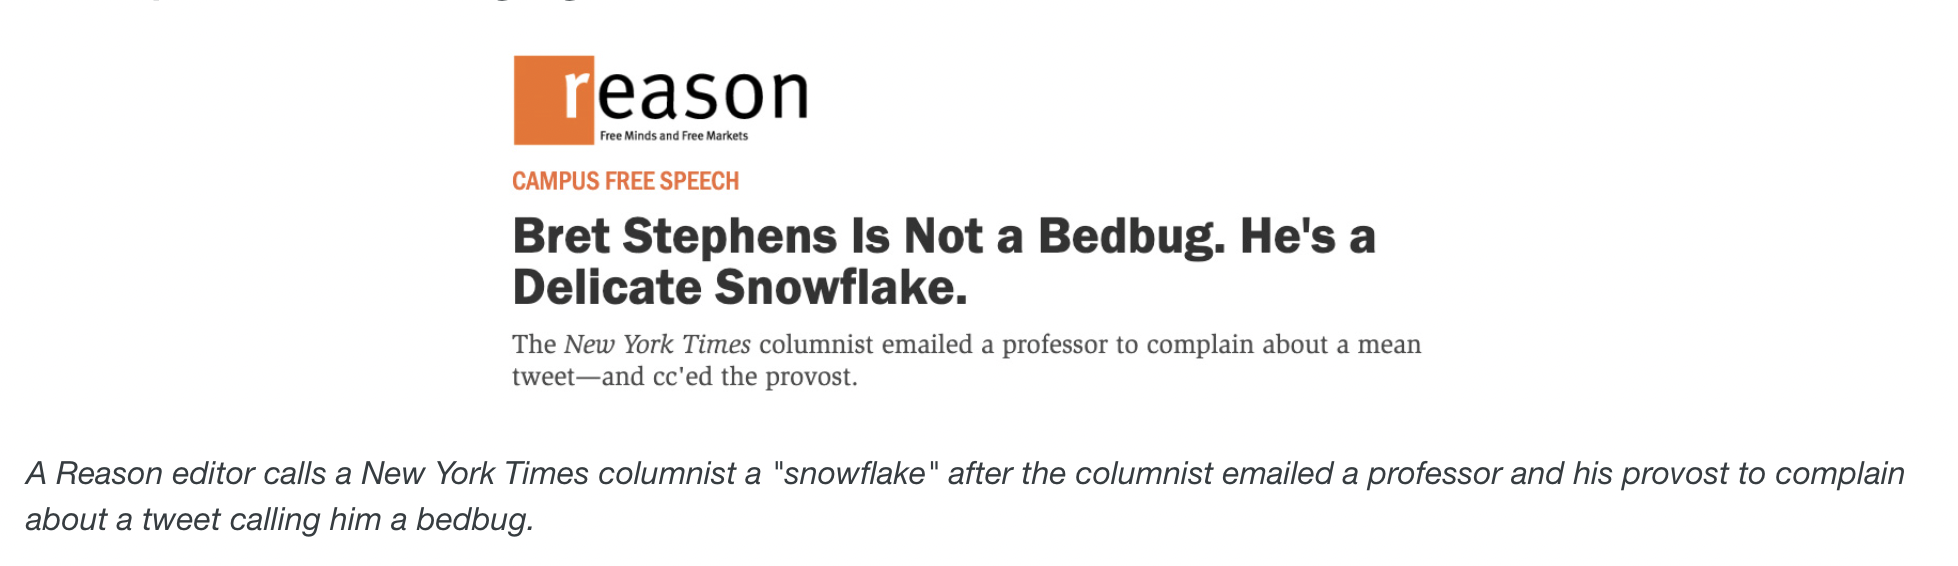
\includegraphics[width=0.95\linewidth]{images/statement_bias_example.png}}
    \caption{Example of phrasing bias (top), spin bias (middle), and statement bias (bottom) \cite{allsides-media-bias-types}}
    \label{fig:bias-examples}
\end{figure}

Figure \ref{fig:bias-examples} shows examples taken from the Allsides website \cite{allsides-media-bias-types} referring to the three types of text-level context bias: phrasing bias, spin bias, and statement bias. \textit{Phrasing bias} is characterised by the use of provocative, inflammatory, or non-neutral language, using words that may evoke specific feelings or emotions in the reader \cite{spinde-2024-taxonomy,hube-2019-neural-biased-language}. The top article snippet in Figure \ref{fig:bias-examples} shows the phrase "it's going to be a bloodbath". The phrase can be considered phrasing bias as it evokes a violent image and may lead readers to perceive the election as extremely chaotic or violent, even though it is not literal. \textit{Spin bias} is introduced when essential information is omitted from the narrative, or when irrelevant information is added instead \cite{spinde-2024-taxonomy}, often as an effort to craft a memorable story \cite{mullainathan-2002-media-bias}. The middle article in Figure \ref{fig:bias-examples} purposefully omitted the crucial information that the number of agencies reporting hate crime incidents has also increased. This creates a false narrative that hate crimes are on the rise, despite the possibility that the increase in reported incidents might be attributed due to higher number of reporting agencies. \textit{Statement bias} occurs when media personnel insert their personal views into the content, resulting in certain news being presented in a manner that is more or less favourable towards a particular view or position \cite{spinde-2024-taxonomy,d-alessio-2000-meta-analysis}. The sentence "He's a delicate snowflake" shown in the example (Figure \ref{fig:bias-examples} bottom article) is clearly a personal opinion of the author of the post.

\begin{figure}[htbp]
    \centering
    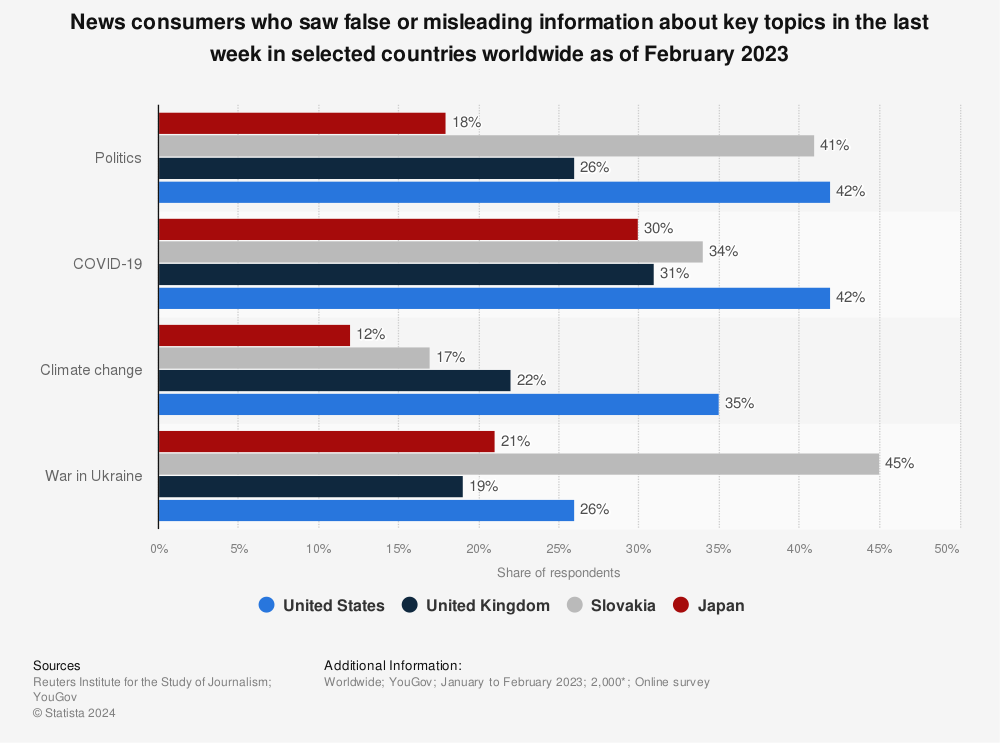
\includegraphics[width=0.7\linewidth]{images/statistic_id1317019_consumers-witnessing-false-information-on-certain-topics-worldwide-2023.png}
    \caption{The rate of news consumers witnessing false or misleading information on several recent key topics in February 2023 \cite{reuters-2023-false-info}}
    \label{fig:consumers-witnessing-false-information-on-certain-topics-worldwide-2023}
\end{figure}


\begin{figure}[htbp]
    \centering
    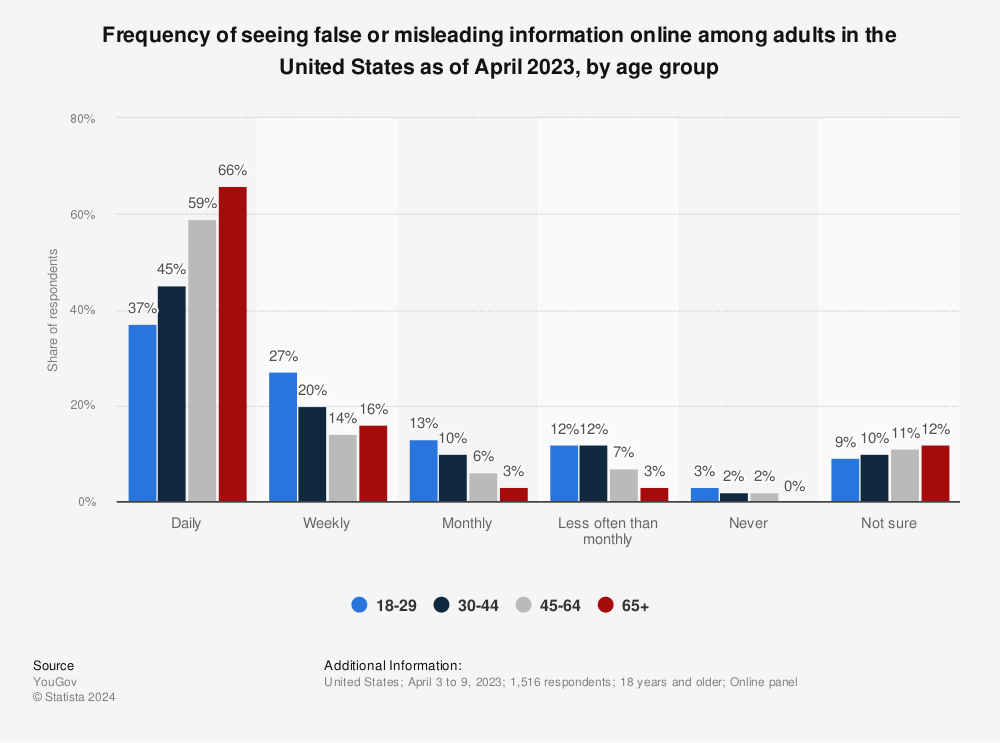
\includegraphics[width=0.7\linewidth]{images/statistic_id1462057_frequency-of-seeing-false-information-online-in-the-us-2023-by-age-group.png}
    \caption{Frequency of seeing false or misleading information online in the United States as of April 2023, by age group \cite{yougov-2023-frequency}}
    \label{fig:frequency-of-seeing-false-information-online-in-the-us-2023-by-age-group}
\end{figure}

Media bias and misinformation are particularly prominent and visible within the United States, compared to other countries. Based on surveys from Reuters \cite{reuters-2023-false-info} and YouGov \cite{yougov-2023-frequency} (Figure \ref{fig:consumers-witnessing-false-information-on-certain-topics-worldwide-2023} and Figure \ref{fig:frequency-of-seeing-false-information-online-in-the-us-2023-by-age-group}), the United States is shown to have the highest rate of encountering false or misleading information related to politics, COVID-19, and climate change. Nearly half of the respondents reported seeing such information in the week prior to the survey, with most adults across all age groups reported seeing false or misleading information on a \textbf{daily} basis.

\begin{figure}[htbp]
    \centering
    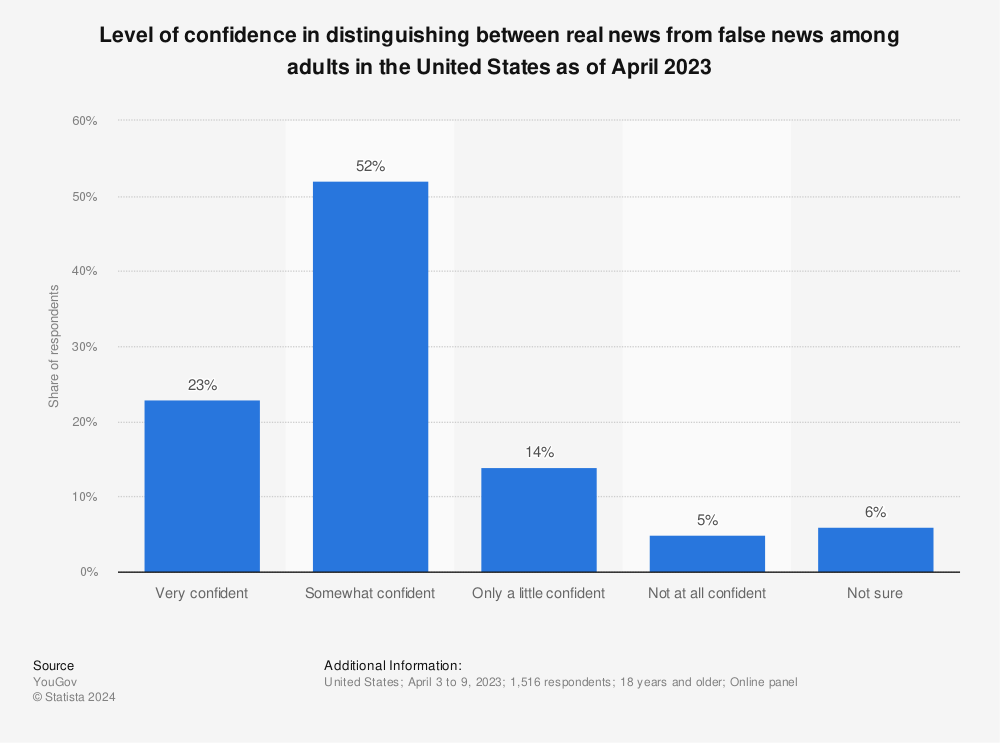
\includegraphics[width=0.7\linewidth]{images/statistic_id657090_ability-to-recognize-false-information-and-news-in-the-us-2023.png}
    \caption{Ability to recognise false information in the US \cite{yougov-2023-confidence}}
    \label{fig:ability-to-recognize-false-information-and-news-in-the-us-2023}
\end{figure}

Another similar survey by YouGov \cite{yougov-2023-confidence} (Figure \ref{fig:ability-to-recognize-false-information-and-news-in-the-us-2023}) shows that as of April 2023, 25\% of respondents feel either only a little confident, not at all confident, or not sure in their ability to distinguish false news from real news in the US. These findings are alarming.

Furthermore, Trust in news media in the US is at an all-time low, declining consistently and significantly over the past 20 years \cite{pew-2021-partisan-divides, gallup-knight-2020-american-views, reuters-2023-digital-news-report}. Approximately half of Americans believe that the media is significantly responsible for the political divisions within the United States, with a growing number of Americans losing faith in the media's objectivity and perceiving it as actively engaging in ideological wars \cite{gallup-knight-2020-american-views}. Reuters Institute also reported less than half of their respondents (40\%) generally trust the majority of news sources, with the US ranked on 29\textsuperscript{th} out of 40 countries (32\%) in terms of trust \cite{reuters-2023-digital-news-report,reuters-2023-trust} (full figure shown in Figure \ref{fig:trustworthiness-of-news-media-worldwide-2023}).

\begin{figure}[htbp]
    \centering
    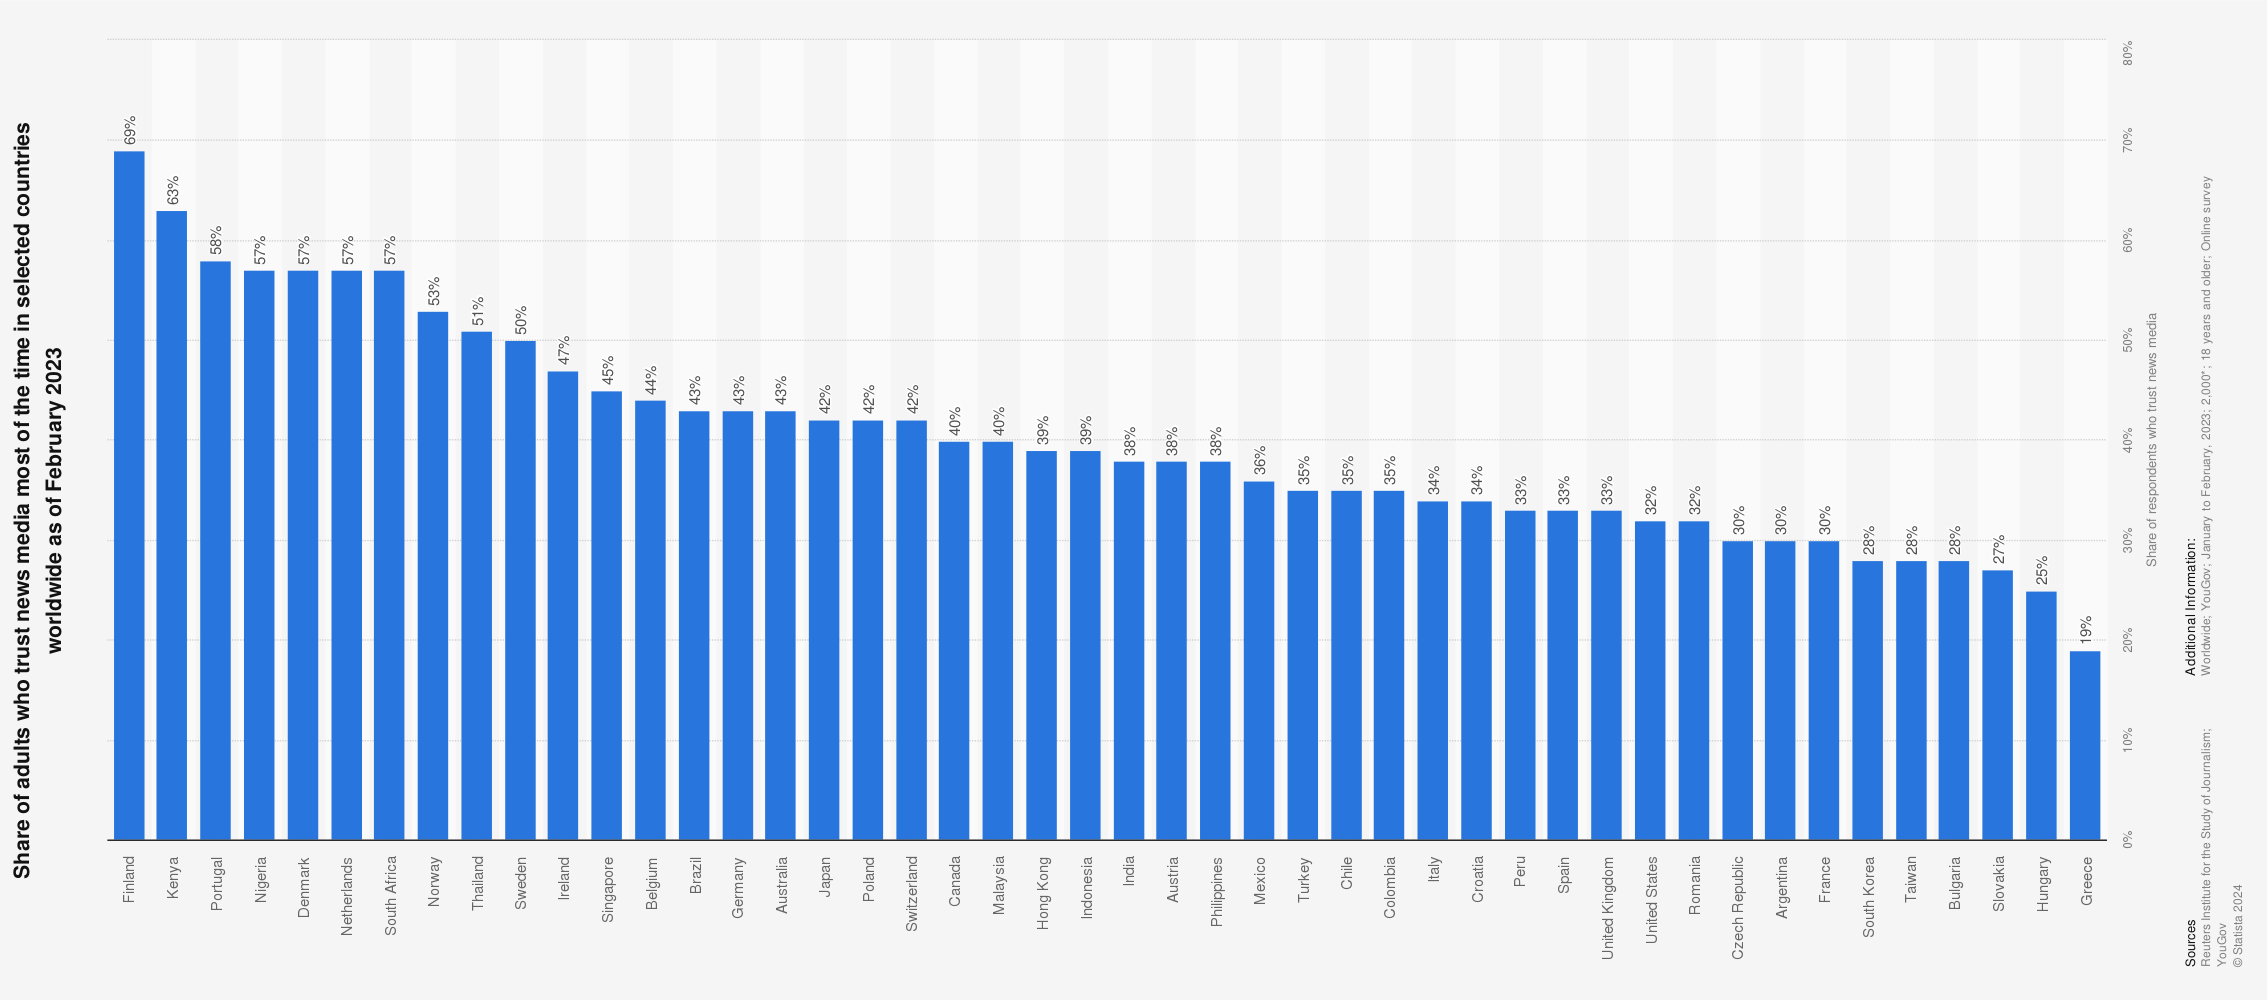
\includegraphics[width=1\linewidth]{images/statistic_id308468_trustworthiness-of-news-media-worldwide-2023.png}
    \caption{Trustworthiness of news media worldwide by country, as of February 2023 \cite{reuters-2023-trust}}
    \label{fig:trustworthiness-of-news-media-worldwide-2023}
\end{figure}

Considering the magnitude of this problem in the US, and given that the majority of research and resources on media bias are typically focused on the US \cite{allsides, adfontes,rodrigo-2024-systematic-review-media-bias}, it is therefore both reasonable and practical for this project to focus on US-based articles and domains.


% Panagopoulos' study \cite{panagopoulos-2020} revealed systemic biases leaning towards Democratic candidates during national and state levels pre-election polls conducted during the 2020 U.S. general election cycle. 

% Rafail et al. \cite{rafail-2018-tea-party} examined 201,678 media documents from Tea Party organizations, Fox News, MSNBC, and 785 newspapers, revealing significant differences in how the Tea Party frames itself compared to how other media sources frame the movement, MSNBC portrays it as the worst aspect of the Republican Party, while Fox News sees it as the best, sharply in contrasts with how activists frame the movement as conservative but not strictly Republican, often clashing with Republican Party goals.

% Readers themselves are not exempt from bias, as they are known to prefer to pick, follow, and consume articles that align with their own beliefs and ideology, an issue known as filter bubble \cite{lim-2018-understanding} or selective exposure \cite{spinde-2024-taxonomy}. This incident reinforces existing biases and limits exposure to diverse perspectives, creating echo chambers that hinder critical thinking and informed decision-making. The combination of media bias and filter bubbles can distort reality, perpetuate misinformation, and deepen societal divisions.

\section{Machine Learning Concepts and Techniques}

\subsection{Text Representation}

\begin{figure}[htbp]
    \centering
    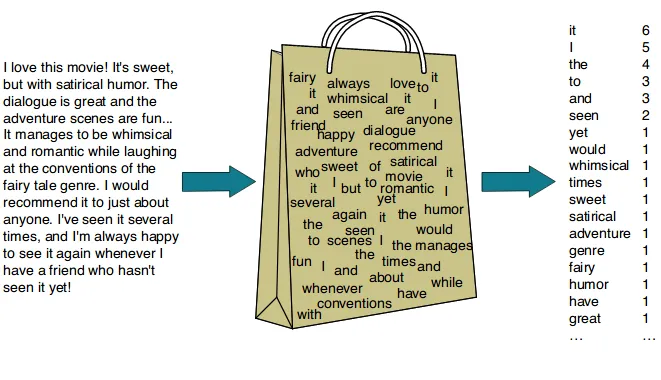
\includegraphics[width=0.7\linewidth]{images/bow_illustration.png}
    \caption{An illustration of how Bag-of-Words work \cite{rahul-2023-bow-medium}}
    \label{fig:bow_illustration}
\end{figure}

\textbf{Bag-of-words (BoW)} is one of the most straightforward techniques to represent text. It works by counting the occurrences of each word for each instance and ignoring the order of the words and grammatical structure \cite{qader-2019-bow}. A simple illustration is shown in Figure \ref{fig:bow_illustration}. The biggest advantage of this technique is that it is computationally cheap and conceptually simple. However, word order and semantics are completely disregarded, and it can be problematic when common words (like stop-words) dominate the representation.

Thus, \textbf{Term Frequency-Inverse Document Frequency (TF-IDF)} can be considered an enhanced version of BoW. It evaluates the importance of a word in a document relative to a collection of documents (corpus). Term Frequency (TF) calculates the number of times a term appears in a document, normalized by the total number of terms in the document. Inverse Document Frequency (IDF) calculates how much information the word provides, i.e., if it is common or rare across all documents. These two calculations will give higher weights on rare and potentially more informative terms rather than frequent words.

Embeddings represent knowledge through low-dimensional vectors that integrate easily into modern machine learning models, which have been a crucial topic in NLP \cite{camacho-collados-2020-embeddings}. This approach gained significant popularity with the introduction of \textit{word2vec} and \textbf{GloVE} \cite{pennington-2014-glove} as methods to generate word embeddings \cite{mikolov-2013-embeddings}, which map each word to a fixed vector (visualised in Figure \ref{fig:word-embeddings}). Embeddings can be extended further to encode sentences and documents instead of words (sentence embeddings and document embeddings). Paragraph vector, or \textit(doc2vec), is a continuation from word2vec, which learns fixed-length feature representations from text segments of varying lengths, including sentences, paragraphs, and documents \cite{mikolov-2014-doc2vec}. However, word embeddings and bag-of-words have been shown to perform better than paragraph vectors models for sentence classification \cite{white-2015-how-well-sentence-embeddings}.

% OOV?

\begin{figure}[htbp]
    \centering
    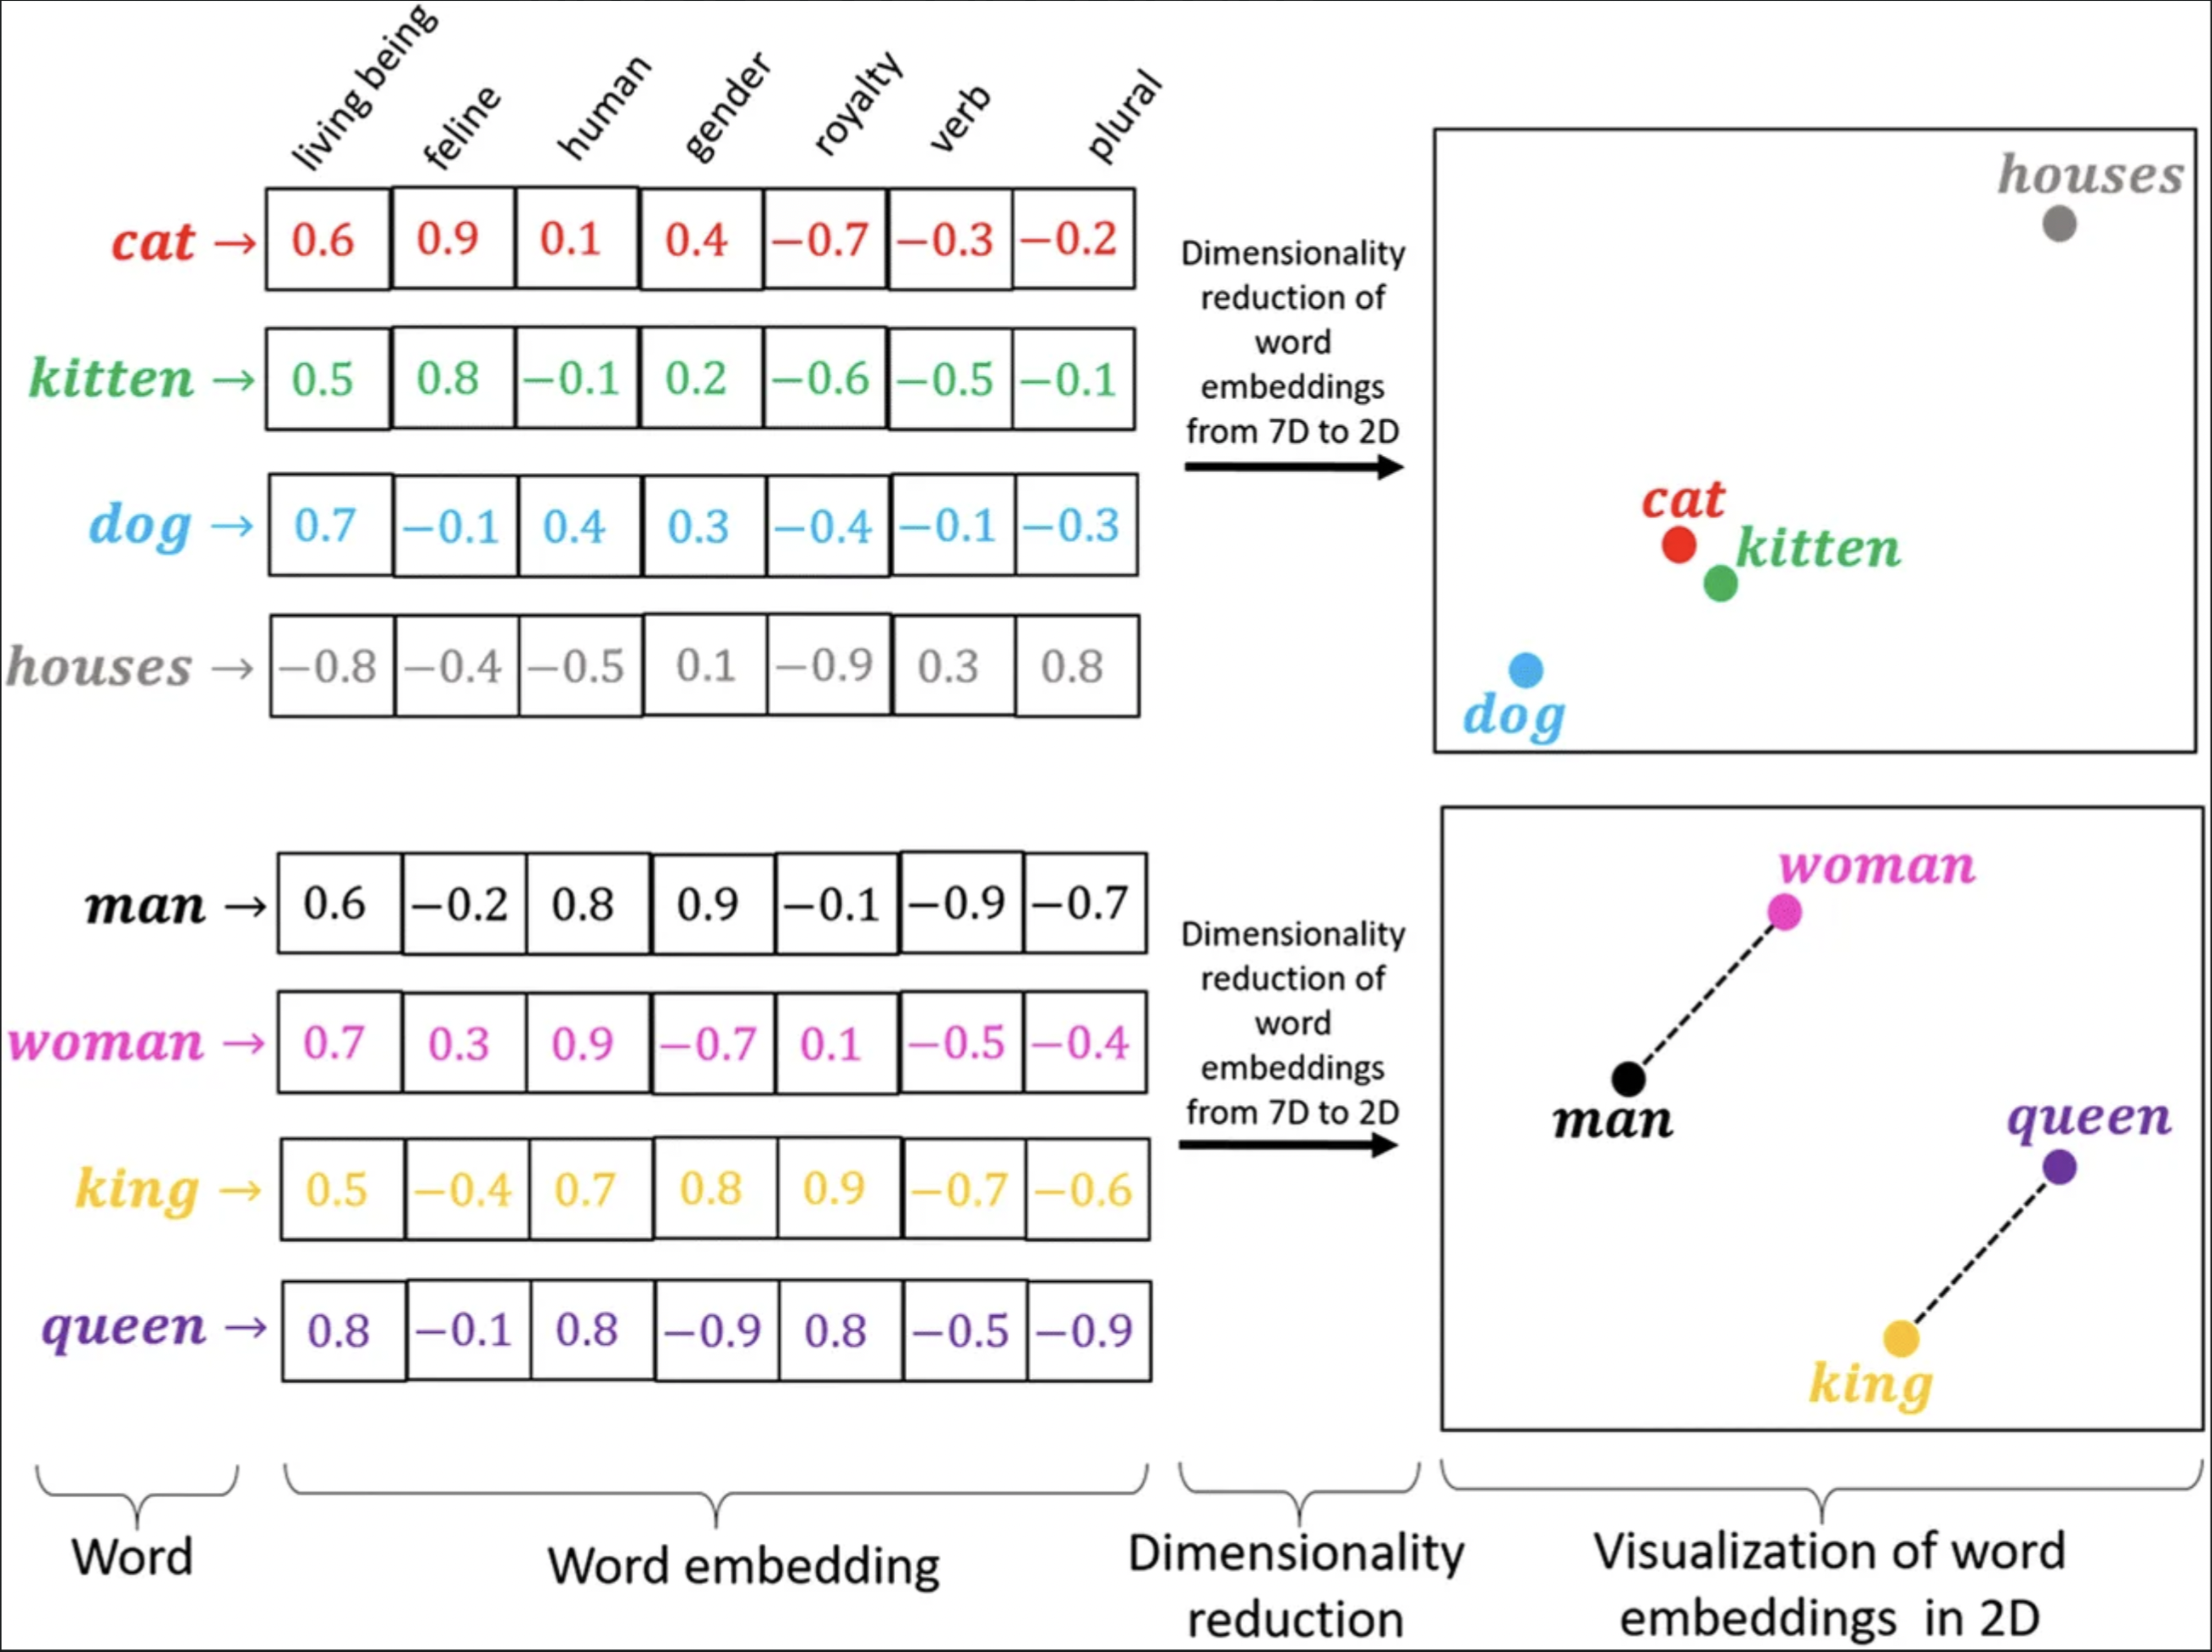
\includegraphics[width=0.8\linewidth]{images/word_embeddings.png}
    \caption{Word embeddings visualisation \cite{narayanan-2019-word-embeddings}}
    \label{fig:word-embeddings}
\end{figure}


Nevertheless, word embeddings have an important limitation. Since every word is mapped into a fixed single vector, word embeddings are considered static or non-contextualised, therefore, unable to distinguish between different meanings of a word \cite{camacho-collados-2020-embeddings}. Words such as 'break,' 'cut,' or 'duck' can have multiple meanings depending on their context, and thus require better modelling to achieve an accurate semantic representation. This problem is solved by contextualised word embeddings, which assign each word with a representation based on its context, allowing it to capture usage in different contexts and encode knowledge that can be transferred across languages \cite{liu-2020-survey-contextual-embeddings}. The embedding is typically encoded dynamically through the use of a pre-trained language model, illustrated in Figure \ref{fig:contextualised-word-embeddings}.

\begin{comment}
Sentence embeddings generated by pre-trained language models often fail to effectively capture the semantic meaning of sentences \cite{li-2020-sentence-embeddings-pretrained-language}
\end{comment}


\begin{figure}[htbp]
    \centering
    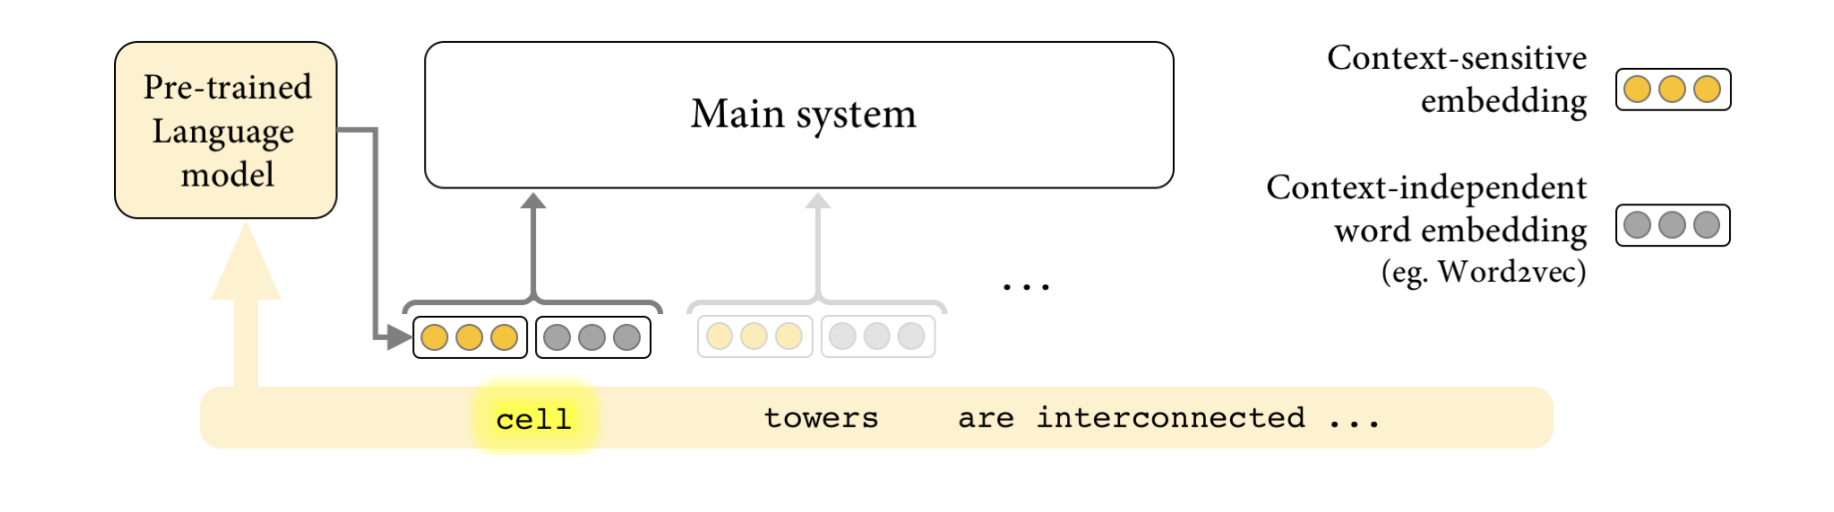
\includegraphics[width=0.9\linewidth]{images/contextualised_word_embeddings.png}
    \caption{An illustration of contextualised word embeddings. A language modelling component analyses the context of the target word (as shown in the figure) and generates its dynamic embedding. \cite{camacho-collados-2020-embeddings}}
    \label{fig:contextualised-word-embeddings}
\end{figure}


\subsection{Neural Networks}

\begin{figure}[htbp]
    \centering
    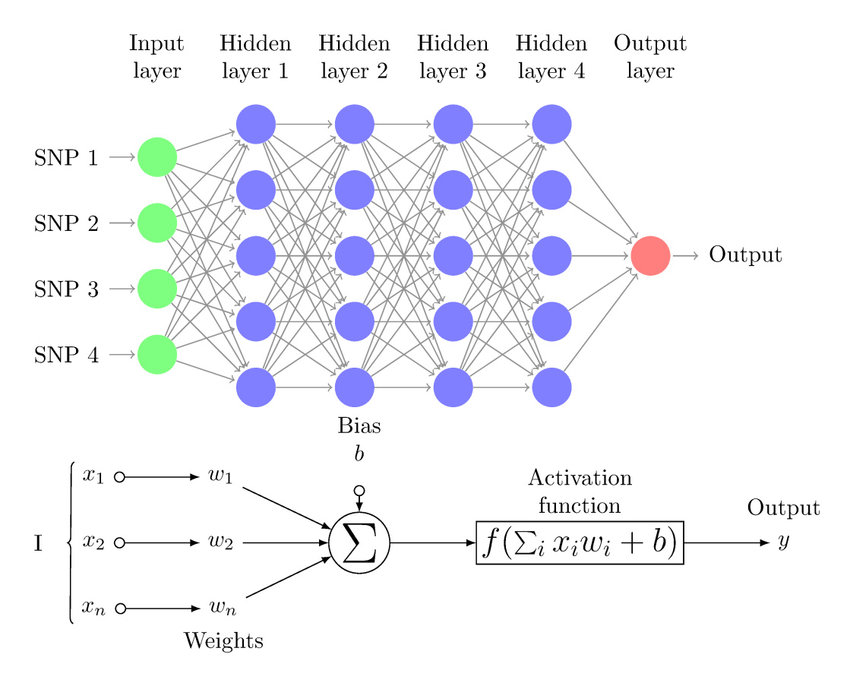
\includegraphics[width=0.9\linewidth]{images/mlp.png}
    \caption{MultiLayer Perceptron visualisation \cite{perez-enciso-2019-guide}}
    \label{fig:mlp}
\end{figure}

Neural Networks or Artificial Neural Networks (ANNs) saw a resurgence of interest after the development of back-propagation algorithm in 1986 \cite{rumelhart-1986-ann}, which made training multi-layer networks feasible and practical. A neural network consists of interconnected nodes called neurons arranged in layers, it utilises the back-propagation algorithm to learn from its errors and continuously improve its performance \cite{aws-neural-network}. These neurons are followed by an activation function, commonly the Rectified Linear Unit (ReLU), which introduces non-linearity into the model and allows the network to learn and represent complex patterns.

\textbf{A MultiLayer Perceptron (MLP)} is a fully connected ANN that consists of single or multiple hidden layers, illustrated in Figure \ref{fig:mlp}. Hidden layers refer to the collection of neurons that are between the input and output layers, transforming data from layer to layer \cite{uzair-2020-hidden-layers}. MLP is widely used due to its ability to introduce non-linearity into the model, allowing the network to approximate complex functions that are beyond the capability of simple linear models \cite{popescue-2009-mlp}.

% \begin{comment}
% The weighted sum (\( \mathbf{z} \)) in a hidden layer of a neural network is computed as follows (Equation \eqref{eq:z}):

% \begin{equation}
%     \label{eq:z}
%     \mathbf{z} = \mathbf{W}\mathbf{x} + \mathbf{b}
% \end{equation} where \( \mathbf{x} \) is the input vector, \( \mathbf{W} \) is the weight matrix, \( \mathbf{b} \) is the bias vector. After computing \( \mathbf{z} \), an activation function \( f \) is applied element-wise to produce the output \( \mathbf{h} \) (Equation \eqref{eq:h}):

% \begin{equation}
%     \label{eq:h}
%     \mathbf{h} = f(\mathbf{z})
% \end{equation}
% \end{comment}

\subsection{Long Short-Term Memory (LSTM)}

\begin{figure}[htbp]
    \centering
    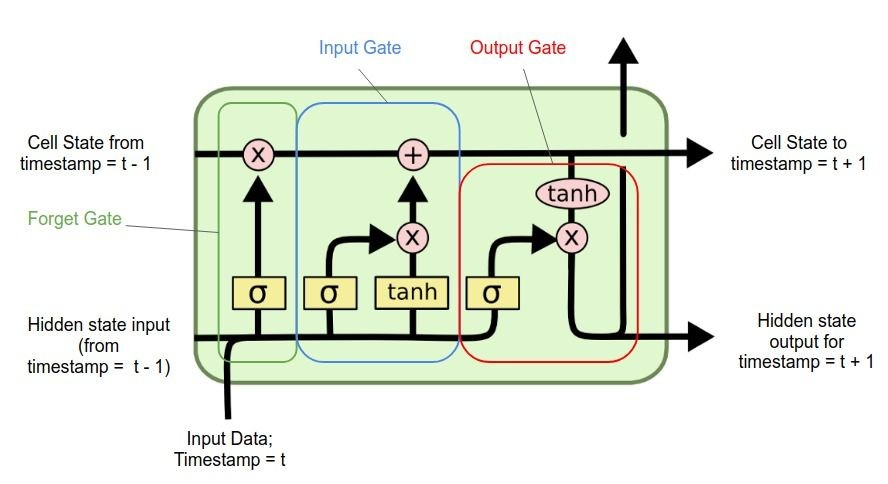
\includegraphics[width=0.8\linewidth]{images/lstm.jpeg}
    \caption{LSTM architecture \cite{rahman-2023-lstm-networks}}
    \label{fig:lstm}
\end{figure}

LSTM \cite{hochreiter-1997-lstm} is a type of Recurrent Neural Network (RNN) architecture designed to address the vanishing gradient problem and capture long-term dependencies in sequential data. It incorporates two fundamental components: memory cells and gates. Memory cells maintain a cell state, which can store information over long sequences and allows the model to retain information for longer durations compared to traditional RNNs. Gates control the flow of information into and out of the memory cell, controlled by sigmoid and tanh activation functions, which regulate the information flow based on the input data and the current state. Figure \ref{fig:lstm} shows the full architecture of a LSTM block.

\subsection{Transformer and Large Language Model (LLM)}

\begin{figure}[htbp]
    \centering
    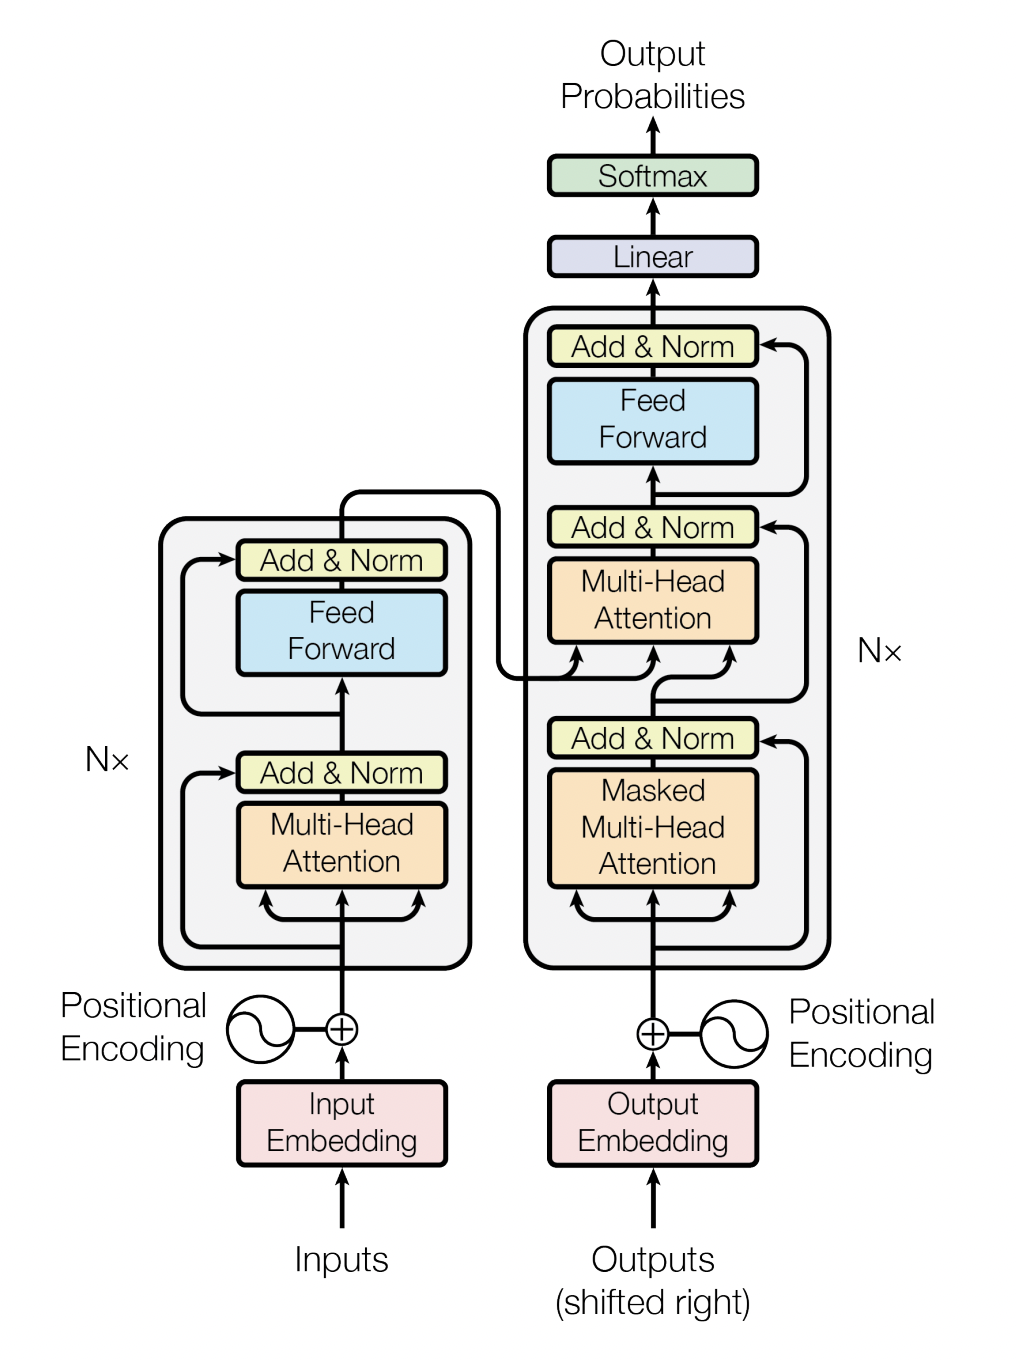
\includegraphics[width=0.65\linewidth]{images/transformer.png}
    \caption{Transformer visualisation \cite{vaswani-2023-attention}}
    \label{fig:transformer}
\end{figure}

The Transformer has become the preferred architecture in NLP, particularly for pre-trained models, due to its capabilities \cite{lin-2022-survey-transformers}. Its architecture relies entirely on attention mechanism to capture global dependencies across input and output sequences, allowing for unprecedented levels of parallelisation instead of sequential processing \cite{vaswani-2023-attention}.

\textbf{Large Language Models (LLMs)} are artificial neural networks that utilise the transformer architecture, designed to understand and generate human language. They are trained on vast amounts of diverse text data using unsupervised learning techniques, often containing millions or even billions of parameters. Two of the most popular and widely used LLMs are \textbf{Bidirectional Encoder Representations from Transformers (BERT)} \cite{devlin-2019-bert}, comprised of 110 million parameters, and GPT, particularly GPT-4 \cite{openai-2024-gpt4}, which is reported to have an astonishing 1.76 trillion parameters, based on a report by SemiAnalysis in 2023 \cite{semianalysis-gpt4}.

As in the BERT original paper \cite{devlin-2019-bert}, pre-trained language representations can be utilised for downstream tasks through two main approaches: \textbf{feature-based} and \textbf{fine-tuning}. Feature-based approach \cite{devlin-2019-bert} leverages a pre-trained model to extract embeddings or features from text and use them as input to other machine learning models for various downstream tasks. Fine-tuning \cite{devlin-2019-bert} adjust the model weights based on the training data for the downstream task, allowing the model to adapt its pre-trained representations to the specific requirements of the task.

Transformers and LLMs have sparked a revolution in the domain of Artificial Intelligence (AI), having achieved remarkable successes across diverse fields such as natural language processing, computer vision, and audio processing \cite{lin-2022-survey-transformers}. They have single-handedly catalysed the emergence of a new era in AI capabilities observed today, predicted to have an even greater influence than the Industrial and digital revolutions combined \cite{makridakis-2017-ai-revolution}.

\begin{figure}[htbp]
    \centering
    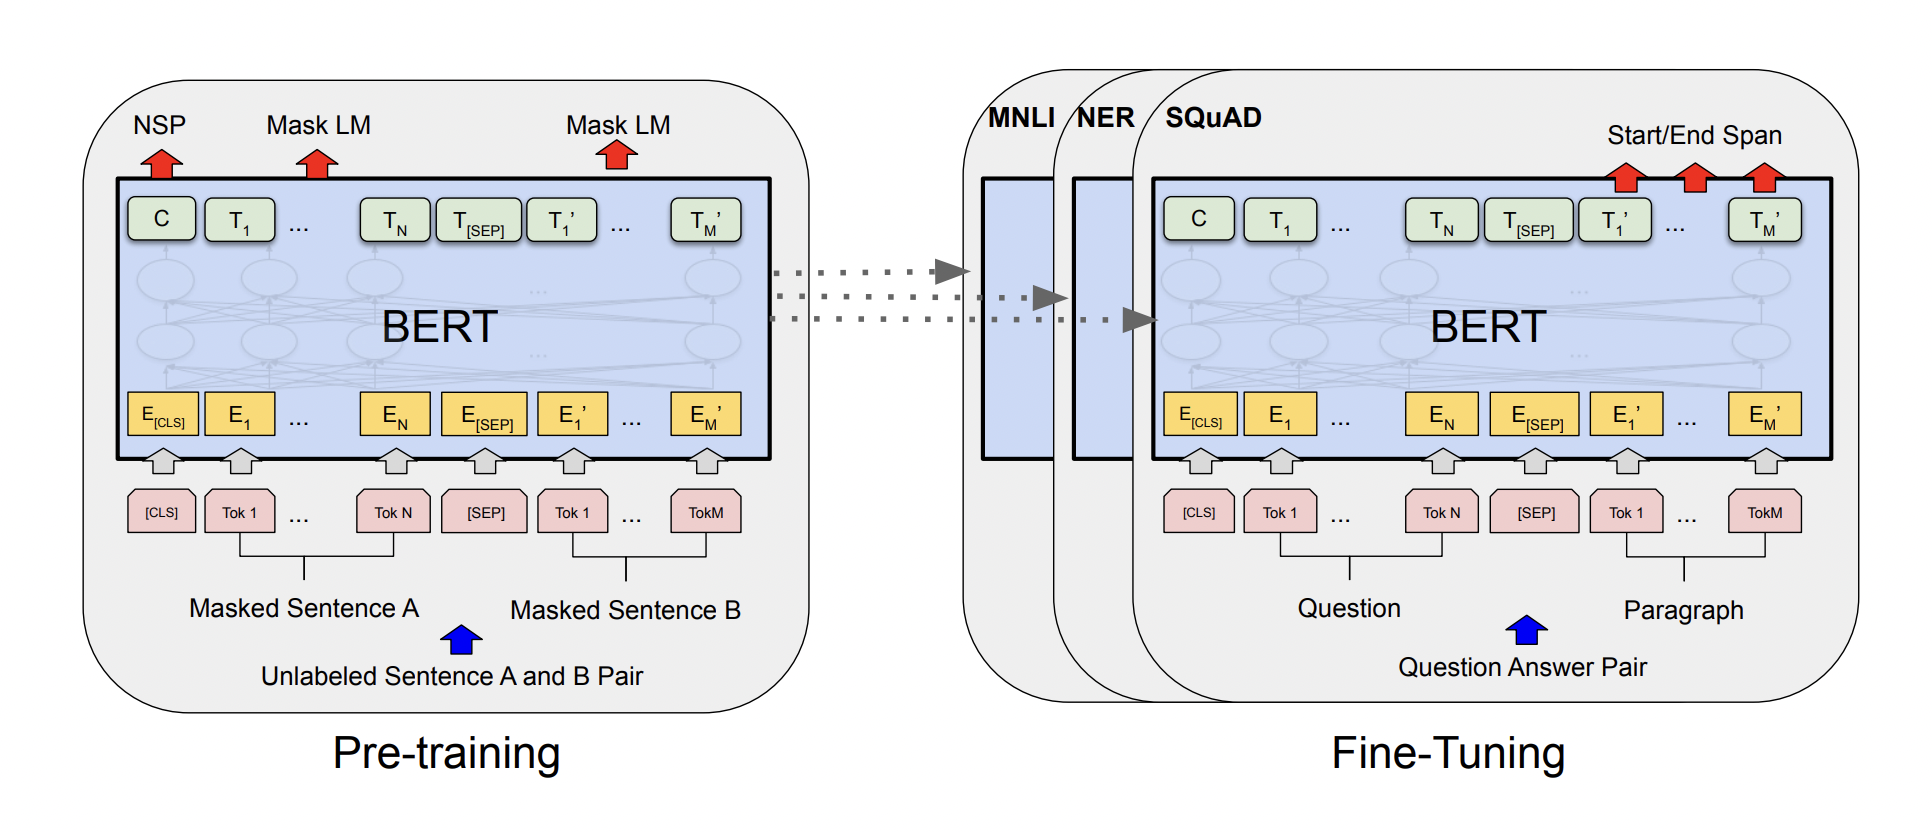
\includegraphics[width=0.9\linewidth]{images/bert_finetuning.png}
    \caption{BERT pre-training and fine-tuning procedures \cite{devlin-2019-bert}}
    \label{fig:bert_finetuning}
\end{figure}

% \begin{comment}
% \begin{equation}
%     \label{eq:attention}
%     \text{Attention}(\mathbf{Q}, \mathbf{K}, \mathbf{V}) = \text{softmax}\left( \frac{\mathbf{Q}\mathbf{K}^\top}{\sqrt{d_k}} \right) \mathbf{V}
% \end{equation}

% \begin{equation}
%     \label{eq:multihead}
%     \text{MultiHead}(\mathbf{Q}, \mathbf{K}, \mathbf{V}) = \text{Concat}(\text{head}_1, \ldots, \text{head}_h) \mathbf{W}^O
% \end{equation}
% where
% \[
%     \text{head}_i = \text{Attention}(\mathbf{Q} \mathbf{W}^Q_i, \mathbf{K} \mathbf{W}^K_i, \mathbf{V} \mathbf{W}^V_i)
% \]
% \end{comment}

\subsection{MAGPIE and DA-RoBERTa}

\begin{figure}[htbp]
    \centering
    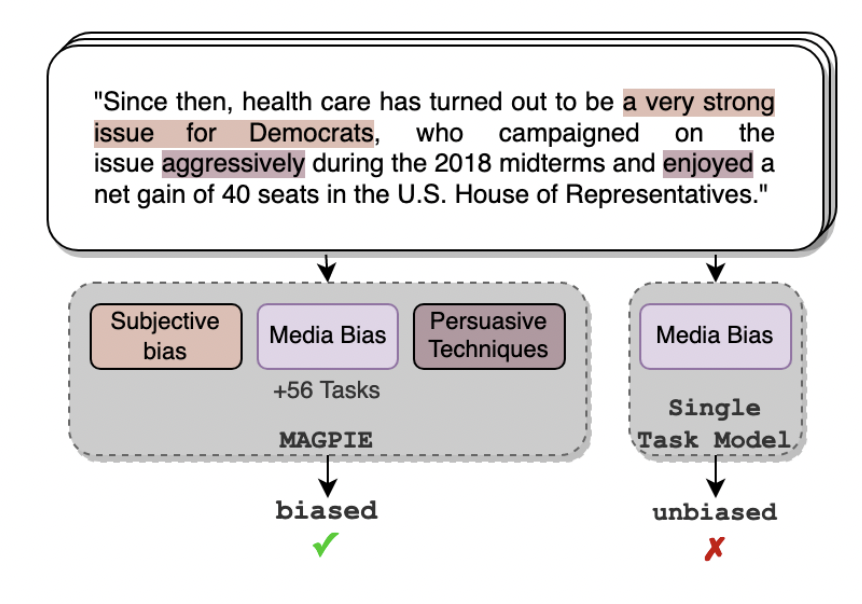
\includegraphics[width=0.7\linewidth]{images/magpie.png}
    \caption{MAGPIE containing a pre-trained representation of various biases \cite{horych-2024-magpie}.}
    \label{fig:magpie}
\end{figure}

\textbf{MAGPIE} \cite{horych-2024-magpie} is a large-scale, RoBERTa-based, multitask pre-training approach specifically designed for media bias detection, pre-fine-tuned on fifty-nine bias-related tasks covering a broad spectrum of biases. Pre-fine-tuning is a large-scale training phase situated between language model pre-training and fine-tuning. It involves extensive multitask learning (MTL) \cite{caruana-1997-mtl} and aims to foster the development of representations that generalise more effectively across various tasks \cite{aghajanyan-2021-muppet}. Pre-fine-tuning allows multitask-approach such as MAGPIE to generalise better on various tasks related to media bias, enabling better performance on these tasks compared to single-task RoBERTa approach \cite{horych-2024-magpie}.

\textbf{DA-RoBERTa} (Domain-Adaptive-RoBERTa) \cite{krieger-2022-domain} is defined as SOTA transformer-based model, pre-trained and tailored for the media bias domain which identify sentence-level bias.

Unfortunately, both MAGPIE and DA-RoBERTa are trained for sentence-level bias and output binary classification (biased or unbiased), therefore unable to be directly fine-tuned for article-level media bias classification task. However, the model and its feature representations can still be utilised for a feature-based approach \cite{devlin-2019-bert}, leveraging the models' knowledge in media bias domain.


\subsection{Chunking and Hierarchical Techniques}

\begin{figure}[htbp]
    \centering
    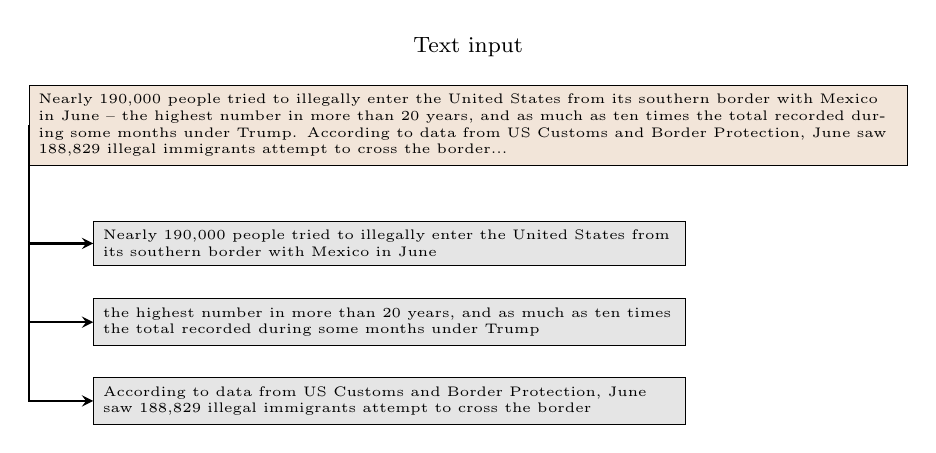
\begin{tikzpicture}
        \tikzstyle{arrow} = [thick,->,>=stealth]
        \tikzstyle{chunk} = [rectangle, draw, fill=gray!20, font=\tiny, text width=0.6\linewidth, align=left]
        \tikzstyle{label} = [text centered,font=\footnotesize]

        \node[label] at (0, 1) {Text input};
        \node (input) [draw, align=left, text width=0.9\linewidth, font=\tiny, fill=brown!20] at (0, 0) {Nearly 190,000 people tried to illegally enter the United States from its southern border with Mexico in June – the highest number in more than 20 years, and as much as ten times the total recorded during some months under Trump. According to data from US Customs and Border Protection, June saw 188,829 illegal immigrants attempt to cross the border...};

        \node[chunk] (chunk1) [draw] at (-1, -1.5) {Nearly 190,000 people tried to illegally enter the United States from its southern border with Mexico in June};
        \node[chunk] (chunk2) [draw] at (-1, -2.5) {the highest number in more than 20 years, and as much as ten times the total recorded during some months under Trump};
        \node[chunk] (chunk3) [draw] at (-1, -3.5) {According to data from US Customs and Border Protection, June saw 188,829 illegal immigrants attempt to cross the border};

        \draw[arrow] (input.west) |- (chunk1.west);
        \draw[arrow] (input.west) |- (chunk2.west);
        \draw[arrow] (input.west) |- (chunk3.west);
    \end{tikzpicture}
    \caption{Illustration of chunking}
    \label{fig:chunking}
\end{figure}


\textbf{Chunking} is a technique used to break down text into smaller, more manageable units. This technique can be applied to segment documents into smaller paragraphs or sentences, as illustrated in Figure \ref{fig:chunking}, facilitating more efficient processing and analysis. \textbf{Hierarchical models} \cite{sun-2020-fine-tune} incorporate multiple levels of abstraction or granularity to capture complex relationships within data. These models are particularly useful when dealing with structured data that naturally falls into a hierarchical organisation, such as documents composed of paragraphs and sentences. Furthermore, \textbf{hierarchical transformer model} is a variant of the transformer architecture that incorporate hierarchical structures to handle long sequences more efficiently. These models process data at different levels, such as sentences within paragraphs, to capture hierarchical relationships. Figure \ref{fig:hi_transformer} shows an example of hierarchical transformer model used to produce document embeddings by utilising sentence-level and word-level information \cite{wu-2021-hi-transformer}.

\begin{figure}[htbp]
    \centering
    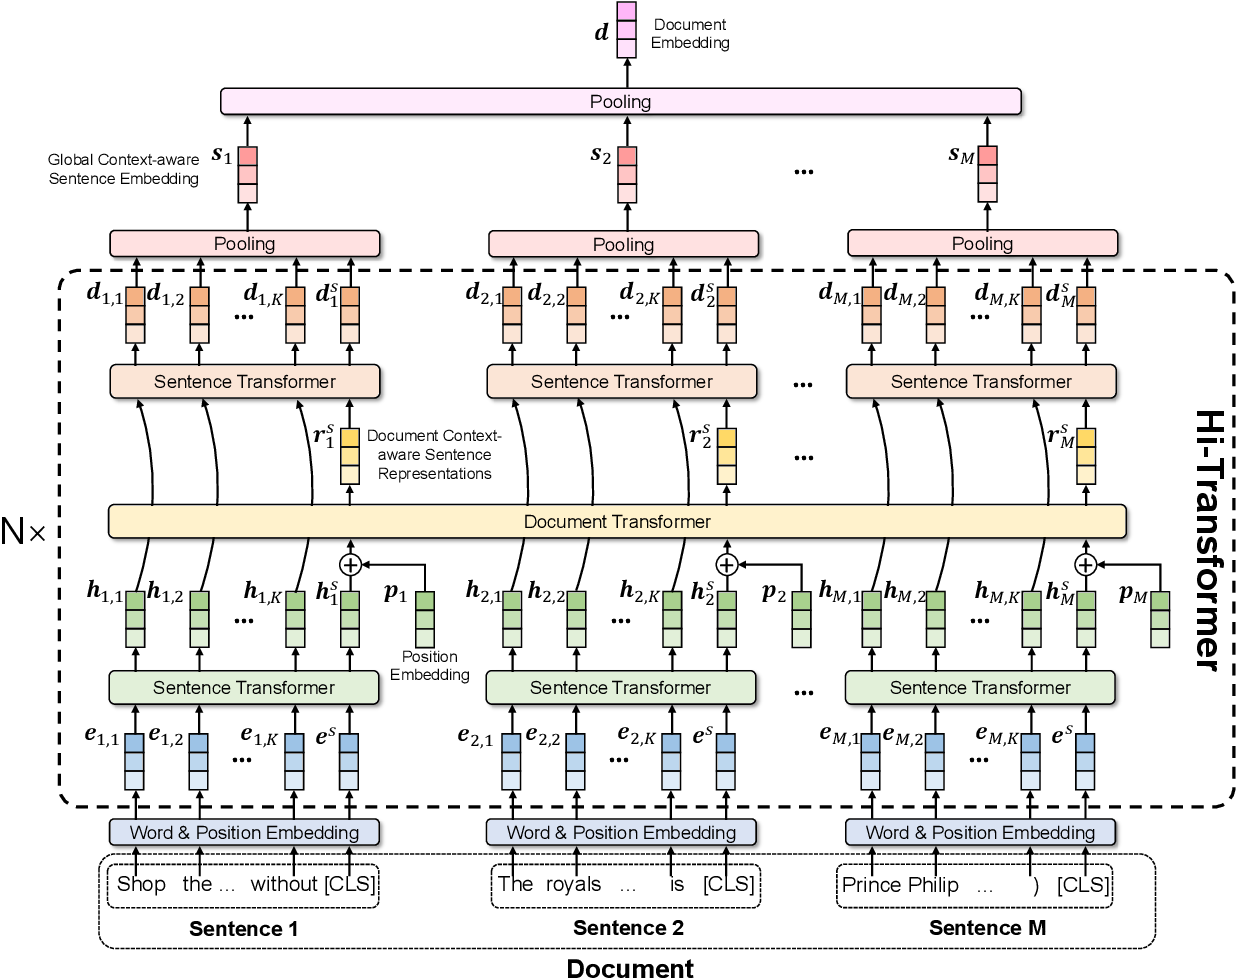
\includegraphics[width=0.9\linewidth]{images/hi_transformer.png}
    \caption{An example of hierarchical transformer model, Hi-Transformer\cite{wu-2021-hi-transformer}, to model long document by incorporating information on sentence and word level.}
    \label{fig:hi_transformer}
\end{figure}


\section{Literature Review}

This section will discuss related works within the domain of document classification, media bias classification, and article-level media bias classification.


\subsection{Document Classification}

Document classification refers to the task of assigning one or more labels to a document from a predefined set of categories \cite{wan-2019-long-length}. This task was first mentioned in 1963 \cite{borko-1963-auto-doc-classification}, with statistical text processing concepts and techniques defined earlier in the 1950s \cite{luhn-1958-business-intelligence-system}. In modern times, Convolutional Neural Networks (CNNs) \cite{afzal-deepdocclassifier,liu-2017-xmlcnn} have been conventionally implemented for this task. However, CNNs have largely been surpassed by more recent methods such as Hierarchical Attention Networks (HAN) \cite{yang-2016-han}, which use word and sentence-level attention to extract significant features from documents, and DocBERT \cite{adhikari-2019-docbert}, which leverages knowledge distillation from the BERT-large model.

A limitation with transformer-based approach for document classification, is that models such as BERT are only able to process a maximum of 512 input tokens \cite{devlin-2019-bert}. Therefore, additional techniques such as chunking or hierarchical approach are necessary to process longer sequences. There exist other LLMs that are designed specifically to handle longer sequences, such as Longformer \cite{beltagy-2020-longformer} and BigBird \cite{zaheer-2021-bigbird}. Longformer utilises a combination of global and local attention mechanisms, while BigBird extends the global and local attention with an additional random attention \cite{zaheer-2021-bigbird,beltagy-2020-longformer}. However, Longformer has been reported to be inconsistent in classification of long documents, performing only notably better than the baseline models (e.g. BERT of the first 512 tokens) on only two datasets \cite{park-2022-efficient}.

Therefore, chunking and hierarchical techniques have been implemented to combat the problem of handling long sequences. Pappagari et al. \cite{pappagari-2019-hierarchical} are among the first to utilise the transformer architecture for long sequences classification, introducing chunking and propagation methods. Su et al. \cite{su-2021-classifying} used chunking methods in a hierarchical transformer model with 'CLS-Pooling' (as also described in \cite{adhikari-2019-docbert}) to extract representations on the document-level for the task of clinical document classification. Khandve et al. \cite{khandve-2022-hierarchical-longdoc} also implemented a hierarchical model by utilising BERT and Bi-LSTM layers for long document classification tasks.


\subsection{Media Bias Classification}

Article classification can be seen as a subset of document classification, focusing primarily on assigning articles into a specific set of categories \cite{dien-2019-article-classification}. In this project articles refer to mostly news pieces published by media outlets. Most news articles typically range between 500 and 1200 words on average \cite{newswhip-2013-article-length}, shorter than many general applications of document classification. Media bias classification refers to the task of analysing and categorising media content to determine the presence and extent of bias. Thus, article-level media bias classification involves performing media bias classification on entire articles rather than on sentences or phrases.

\begin{figure}[htbp]
    \centering
    \fbox{
        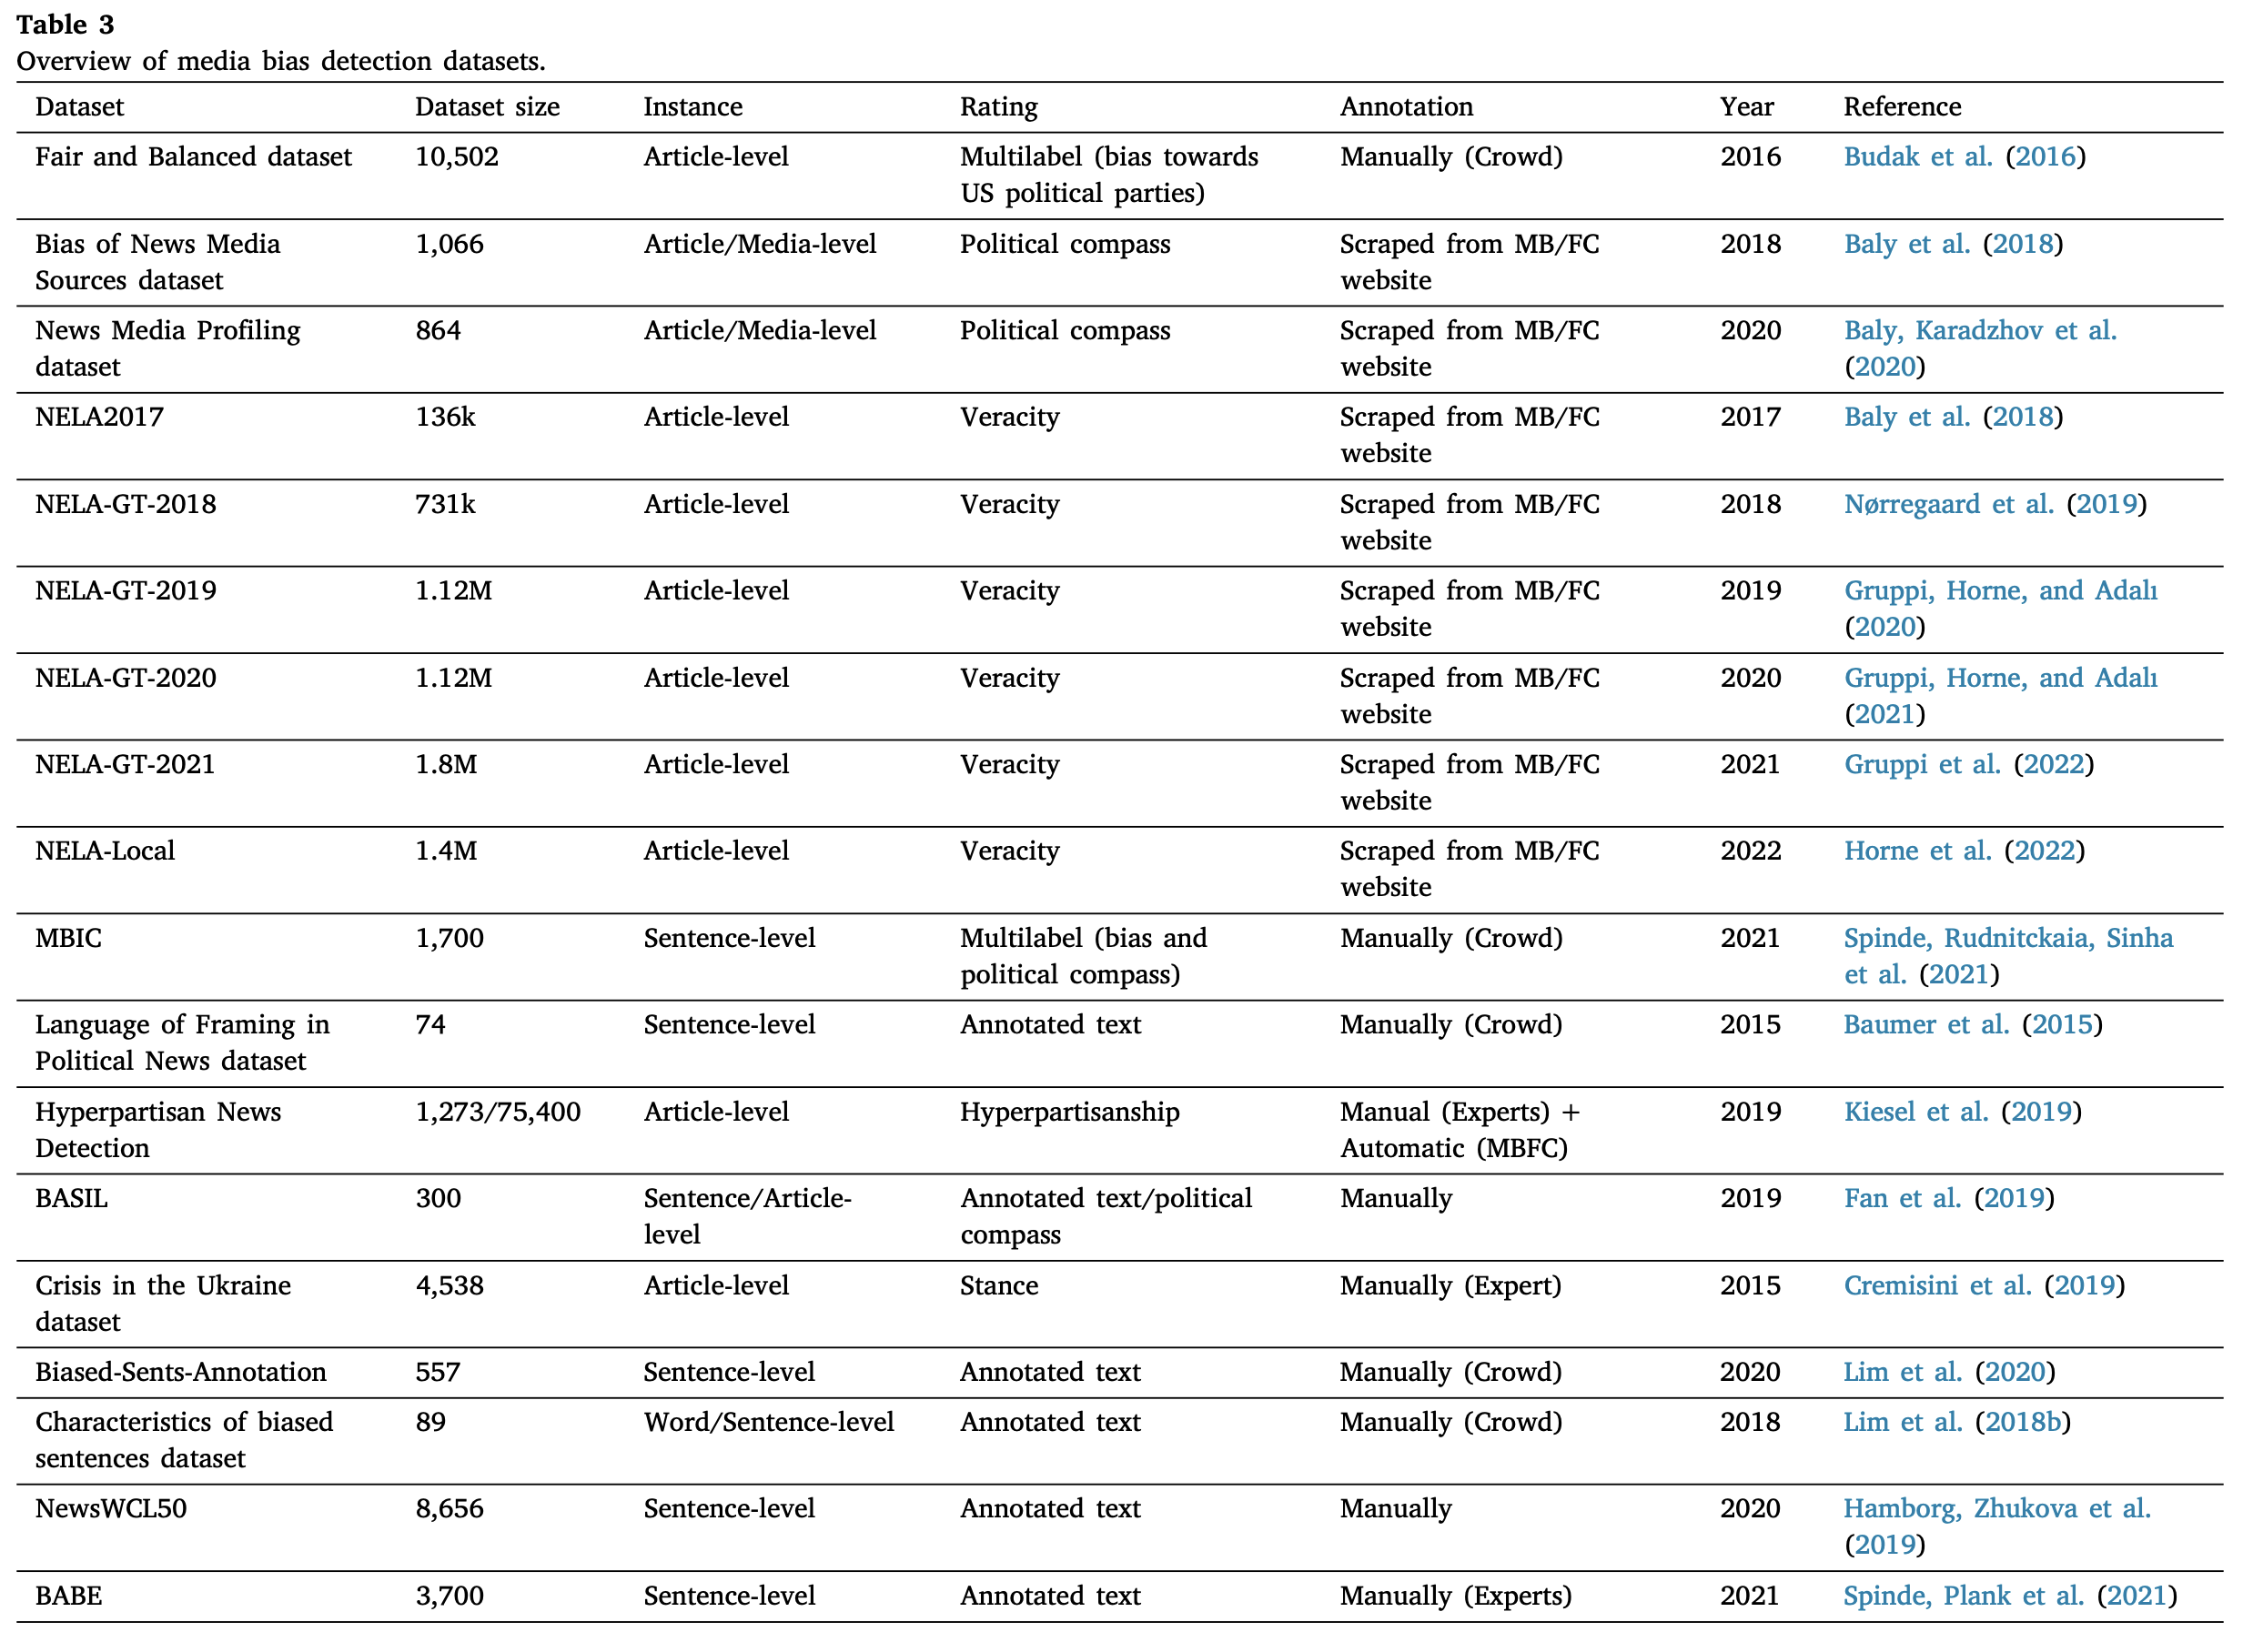
\includegraphics[width=0.9\linewidth]{images/media_bias_dataset_overview.png}}
    \caption{Overview of available media bias datasets \cite{rodrigo-2024-systematic-review-media-bias}}
    \label{fig:media-bias-datasets-overview}
\end{figure}

Current available datasets for article-level and media bias classification often vary in formats or incorporate different types of bias \cite{rodrigo-2024-systematic-review-media-bias} (Figure \ref{fig:media-bias-datasets-overview}). Consequently, it is challenging to compare these datasets directly in terms of their quality and usefulness.

The \textbf{BASIL} dataset \cite{fan-2019-basil} is the most commonly used bias dataset, containing 300 articles with both article-level and phrase-level annotations. The \textbf{NLPCSS} \cite{chen-2020-nlpcss} dataset, with 6,964 articles annotated via Ad Fontes labels, includes article-level textual content with three bias labels (bias, neutral, or unknown).

The \textbf{NELA-GT-2022} dataset \cite{gruppi-2023-nela-gt-2022} includes 1,778,361 articles from 361 outlets, annotated with labels from the MBFC \cite{mbfc} website. Despite its large size, the primary issue with this dataset is the ambiguity of its three labels: reliable, mixed, and unreliable. I argue that these labels lack clarity and fail to provide sufficient information about the annotated articles. The 'mixed' label, in particular, poses a challenge as it is unclear how to interpret articles categorised under this label. This lack of precision in classification undermines the utility of the dataset for rigorous analysis and research purposes. Similarly, the NLPCSS dataset faces the same issue.

The \textbf{BAT} dataset \cite{spinde-2023-bat} which includes 6,345 articles from 321 outlets annotated with Ad Fontes labels. Unlike other datasets, the BAT dataset provides clear and precise labels with its bias reliability scores for articles. However, the dataset lacks the textual content of the articles, requiring further extension by crawling the article content from the respective websites, a process which will be fully described in the next chapter.

Other datasets shown in Figure \ref{fig:media-bias-datasets-overview} either have a political compass rating or are annotated at the sentence level, making them unsuitable for this project.

Past works on media bias classification typically use the BASIL dataset, operating on a sentence-level and outputting binary result (either biased or not) \cite{maab-2023-lexical-bias-detection, maab-2023-target-aware, guo-2022-modeling, van-den-berg-2020-context,lee-2021-unifying,lei-2022-sentence,lei-2024-event-relation,krieger-2022-domain}, complemented by the lack of appropriate and adequate datasets with article-level annotations \cite{demidov-2023-political-bias-classification}.

Consequently, There are only a few existing works on article-level media bias classification, with most works focusing on detecting political bias (leaning-left, right, or centre) or ideology instead of purely media bias. Kulkarni et al. \cite{kulkarni-2018-multi-view} proposed a method that incorporates cues from the title, link structure, and content of articles to predict political ideology. Baly et al. \cite{baly-2020-we-can-detect-your-bias} adversarial media adaptation approach to detect political bias in news articles. Kim and Johnson \cite{kim-johnson-2022-close} proposed an MTL model (CLoSE) that consisted of either a BERT-based or RoBERTa-based encoder, followed by a pooling layer to create a sentence embedding, which is then fed into a classifier to predict political bias. Chen et al. \cite{chen-2020-detecting-media-bias-gaussian} employed a Gaussian mixture model that exploits sentence-level bias information to detect article-level bias. Chen et al.'s definition and approach to media bias closely align with this project; however, it does not incorporate any transformer-based or state-of-the-art (SOTA) methods.


% \begin{comment}
% Furthermore, annotating media bias is not a straightforward task. Traditionally, this is done by hiring experts and journalists to manually read and determine how biased the content is. Here it is important to use multiple annotators to minimise introducing another form of bias towards the dataset. This comes with its own set of challenges as annotators might not always agree on biased text \cite{lim-2018-understanding}. As with \cite{spinde-2021-babe}, annotations are generally compiled and majority voted to achieve the final annotation given a particular text. Moreover, annotators' personal background moderately influenced their decisions and should be taken into consideration when building datasets, along with other factors such as topics, reading news habits, and honest mistakes \cite{spinde-2021-bias-words}. Clearly, this is not a cheap procedure and can act as a bottleneck when building a reliable media bias dataset.

% Alternatively, organisations such as Allsides \cite{allsides} and Ad Fontes \cite{adfontes} have their own experts and annotations which can be crawled and exploited. Several papers and datasets \cite{spinde-2023-bat,chen-2020-nlpcss,kulkarni-2018-multi-view} have utilised this approach. However, since these datasets depend on manual labelling from third-party organisations, the selection of articles likely also introduces bias into the dataset \cite{spinde-2023-bat}.

% \end{comment}



%%% Local Variables: 
%%% mode: latex
%%% TeX-master: "thesis"
%%% End: 
\chapter{Dataset Reconstruction and Analysis}
\label{cha:3}

This chapter discusses the chosen dataset for this study, the BAT dataset. It includes details on the dataset's analysis, cleaning, and reconstruction through crawling article contents.

\section{The BAT dataset} \label{bat-characteristics}

The BAT dataset \cite{spinde-2023-bat} contains 6,345 rows of manually labelled news articles published by 255 English-speaking news outlets (US-based), originally scraped from Ad Fontes Media's website. Articles in the dataset encompassed a wide range of topics such as COVID-19, politics, and lifestyle. This dataset was chosen for this project primarily because of its political bias and reliability scores, which provide a clear and useful label for classifying media bias at the article level.

The political bias score measures the extent of political influence, ranging from -42 (most extreme left) to +42 (most extreme right), reflecting the article's truthfulness, with values ranging from 0 (least reliable, containing inaccurate or fabricated information) to 64 (most reliable, original fact reporting) \cite{adfontes-bias-reliability}. The reliability score evaluates original fact reporting to analysis, opinion, propaganda, and inaccurate/fabricated information, with scores above 40 generally considered good and scores below 24 typically seen as problematic, scores between 24 and 40 suggest a variety of factors, including a strong presence of opinion and analysis or significant variability in reliability across different articles \cite{adfontes-bias-reliability}.

Ad Fontes rates articles using a politically balanced panel consisting of at least three analysts representing right-leaning, centrist, and left-leaning perspectives. The scores from each analyst are compared, and any discrepancies are discussed and adjusted if necessary, before averaging to obtain the final rating \cite{adfontes-methodology}. No further information can be found regarding their specific values and range of these rating, it can be safely assumed that this is an inherent part of their algorithms and methodology.

The reliability score is selected as the label in this project because it measures truthfulness and original fact reporting. Articles with high reliability scores typically do not exhibit any textual-level biases, such as phrasing bias, spin bias, or statement bias, as described in Chapter \ref{cha:2}.

\begin{figure}[htbp]
    \centering
    \begin{minipage}{1\linewidth}
        \begin{center}
            \small{\textbf{Trenton police officer takes own life in Plainsboro parking lot, officials say}}
        \end{center}
        \scriptsize{
            A veteran Trenton police officer took his own life in a parking lot Wednesday, officials said. Sgt. Daniel Pagnotta, a 21-year-veteran of the department, died this morning in Plainsboro, according to a city spokesman.“Beloved by everyone in the Trenton Police Department, he was devoted to Trenton and police work,” Mayor Reed Gusciora said in a statement. The statement described Pagnotta as a devoted husband and father of two who loved soccer and making people laugh. His father, also named Dan, is a retired Trenton police officer.“Dan was proud to continue a legacy of law enforcement in his family,” Gusciora said. “Dan and his family are on our minds and in our hearts. He will be dearly missed.”}
    \end{minipage}
    \caption{Example of a non-biased article, reliability score: 57.67}
    \label{fig:example-nonbiased-article-1}
\end{figure}

\begin{figure}[htbp]
    \centering
    \begin{minipage}{1\linewidth}
        \begin{center}
            \small{\textbf{Army Rejects Mike Flynn’s Call For Trump To Declare Martial Law And Overturn The Election}}
        \end{center}
        \scriptsize{
            After Mike Flynn called for Trump to declare martial law and overturn the election, Army leadership flatly rejected the idea. The Army response to Flynn’s fascist idea was to reject it: The military has made it very clear that they will not be participating in any last-ditch attempts by Trump to destroy democracy to stay in power. Flynn’s idea that Trump should overturn the election shows that Trump and his associates have always been anti-democratic. They don’t respect democracy or view it as their role to uphold and promote democratic institutions in the United States. There is not going to be any declaration of martial law. Trump isn’t going to overturn the election. Trump is not going to get help from the military to stay in power. The soon to be former president was the face of the fascist threat, but he has converted the Republican Party into an anti-democratic movement for autocracy. Donald Trump lost, but the authoritarian impulse behind Trumpism still must be defeated for democracy in the United States to be saved.}
    \end{minipage}
    \caption{Example of a non-biased article, reliability score: 30.0}
    \label{fig:example-mixed-biased-article-1}
\end{figure}

\begin{figure}[htbp]
    \centering
    \begin{minipage}{1\linewidth}
        \begin{center}
            \small{\textbf{Is the FBI corrupt beyond repair?}}
        \end{center}
        \scriptsize{
            Last week, the most recent slap in the face to the American people came in the form of a corrupt FBI lawyer getting a fine less than seatbelt ticket for falsifying documents to violate the civil rights of American citizens. Unfortunately, this is the latest in a laundry list of issues with the FBI. The most glaring problem with the FBI is its actions during the Russia Collusion hoax. The FBI allowed itself to become the enforcement arm of the Democratic Party. There is a slim chance the law enforcement agency did not know it was being used initially, but it had to know it was being used shortly after the 2016 election...
        }
    \end{minipage}
    \caption{Example of a biased article, reliability score: 6.67}
    \label{fig:example-biased-article-1}
\end{figure}

An example of a highly-rated article can be seen in Figure \ref{fig:example-nonbiased-article-1}. The article reports only factual information regarding the event and includes statements from people related to the incident. It contains no journalist opinions or political innuendos. In contrast, an example of a low-rated article can be seen in Figure \ref{fig:example-biased-article-1}. The article refers to the event as "the most recent slap in the face," which exemplifies phrasing bias. Additionally, the author's negative view of the FBI is evident, indicating a statement bias. Lastly, Figure \ref{fig:example-mixed-biased-article-1} shows an article that is rated in the middle quartile with a reliability score of 30.0. The article uses strong language, such as "fascist," and makes a broad assumption, claiming that Trump is anti-democratic. While the points raised in the article may have elements of truth, the way they are presented lacks balance and neutrality.

\section{Reconstruction}

The original BAT dataset contains the titles and URLs of articles but missing the full content. Therefore, it is necessary to crawl the websites to retrieve the complete article content. To address this, a Python script was developed to iteratively visit each URL in the dataset and extract the textual content. The initial round yielded 5,270 articles from the original 6,345 articles, with substantial data loss attributed to unavailable websites, missing articles, and broken links. Additionally, some pages could not be crawled by the script due to structural differences and had to be manually copied and pasted.

Subsequently, a second round of data retrieval was conducted by re-examining 1,075 articles that were not successfully crawled in the initial round. Each of these cases was individually investigated: missing articles were sought through public archives, broken links were repaired, using proxies to bypass geographical restrictions. Articles that were successfully retrieved were added to the dataset, resulting in an additional 226 articles. Thus, the final dataset contains 5,497 articles.

The extracted text contains noise, which upon inspection is categorised into two different types: \textbf{word-level noise} and \textbf{phrase-level noise} as illustrated in Table \ref{table:conjoined_words} and Table \ref{table:noise_phrases}. Word-level noise includes typing errors and conjoined words, mostly attributed to word links or texts with unusual HTML format that are difficult to cleanly extract. Phrase-level noises are attributed to extraneous content such as author information, subscription prompts, and donation appeals within the article text.

\begin{table}[htbp]
    \centering
    \small
    \begin{tabular}{| c | c | c |}
        \hline
        Newsreported           & saidon        & admittedthat       \\
        \hline
        TheNational            & 2021According & theirwithholdingis \\
        \hline
        statementthat          & DakotaToni    & Democrattoldthe    \\
        \hline
        DemocratsThe           & whatreporter  & PresidentVladimir  \\
        \hline
        Bidensaid              & whohas        & theDemocrats       \\
        \hline
        includingthe           & saidRep       & toreopen           \\
        \hline
        2021Trump              & Americanswho  & duringhis          \\
        \hline
        thecoronaviruspandemic & toMissouri    & toReuters          \\
        \hline
        haspreviously          & Postcolumnist & 2ndAmendment       \\
        \hline
    \end{tabular}
    \caption{Example of word-level noise, over sixty-thousand occurrences are found within the dataset article contents}
    \label{table:conjoined_words}
\end{table}

\begin{table}[htbp]
    \centering
    \scriptsize
    \begin{tabular}{| l |}
        \hline
        By submitting your email, you agree to our Terms and Privacy...                                        \\
        \hline
        ByChris MurphyByNick BiltonByErin Vanderhoof                                                           \\
        \hline
        Get a brief on the top business stories of the week, plus CEO interviews...                            \\
        \hline
        Kevin Winter/Getty Images                                                                              \\
        \hline
        Subscribe to our free News Alerts newsletter. Want more of our free, weekly newsletters in your inbox? \\
        \hline
        Join the 3,900+ MTFP members who believe in the power of independent news...                           \\
        \hline
        We're hiring! Please take a look at the new openings in our newsroom...                                \\
        \hline
        BYPASS THE CENSORSSign up to get unfiltered news delivered straight to your inbox                      \\
        \hline
        RealClear PoliticsLiz Peek writes about business and government. Submit a letter...                    \\
        \hline
        Follow Stephen Robinson onTwitter. Want to just donate once?                                           \\
        \hline
        At Vox, we believe that clarity is power, and that power shouldn’t only be available to those...       \\
        \hline
    \end{tabular}
    \caption{Examples of phrase noises, mostly subscription and donation prompts, that were inadvertently crawled into the article content.}
    \label{table:noise_phrases}
\end{table}

To identify word-level and phrase-level noises, the entire content of every article in the dataset was combined and tokenised, then matched with an English word list \cite{dwyl-english-words}, generating an error list that includes words found in the articles but not present in the dictionary. Entries in this error list were manually inspected, prioritising commonly occurring items. Based on these findings, scripts were developed to address both word-level and phrase-level noise. This process was iteratively repeated to correct as many issues as possible. However, due to project time constraints, it was impractical to resolve all identified and potential noises, which would have required extensive time and manual effort.

A total of 5,761 word-level noises were corrected, and 625 phrase-level noises were identified and stripped from article contents. The total of word-level noises that exist within the dataset is predicted to be over sixty-thousands occurrences, based on the error list. Pseudocode of the scripts can be seen in Algorithm \ref{alg:phrase_level_noise_fix} and \ref{alg:word_level_noise_fix} (Appendix \ref{app:A}).


\begin{table}[htbp]
    \centering
    \footnotesize
    \begin{tabular}{| c | c | c | c | c |}
        \hline                            \textbf{Method} & \textbf{Class}     & \textbf{Precision} & \textbf{Recall} & \textbf{F1} \\\cline{1-5}

        \multirow{5}{*}{BERT FT, before noise cleaning}   & Problematic        & 0.43               & 0.37            & 0.40        \\
                                                          & Questionable       & 0.33               & 0.39            & 0.36        \\
                                                          & Generally Reliable & 0.39               & 0.53            & 0.45        \\
                                                          & Reliable           & 0.91               & 0.81            & 0.86        \\\cline{2-5}
                                                          & Overall            & 0.7379             & 0.6994          & 0.7147      \\
        \hline
        \multirow{5}{*}{BERT FT, after noise cleaning}    & Problematic        & 0.43               & 0.44            & 0.44        \\
                                                          & Questionable       & 0.29               & 0.39            & 0.33        \\
                                                          & Generally Reliable & 0.44               & 0.48            & 0.46        \\
                                                          & Reliable           & 0.90               & 0.83            & 0.86        \\\cline{2-5}
                                                          & Overall            & 0.7359             & 0.7065          & 0.7193      \\
        \hline
    \end{tabular}
    \caption{Performance before and after noise cleaning of BERT fine-tuning}
    \label{table:noise_performance_comparison}
\end{table}

To evaluate the effects of the noise-cleaning procedure, a simple BERT fine-tuning approach is performed on the dataset with and without noise. As shown in Table \ref{table:noise_performance_comparison}, the cleaned dataset results in a slight improvement in both recall and F1 scores, along with a minor reduction in precision. This outcome is expected, as only a portion of the noise in the dataset was addressed. Continuation in further noise cleaning is projected to yield more pronounced improvements in performance.


\section{Analysis}

\begin{figure}[htbp]
    \centering
    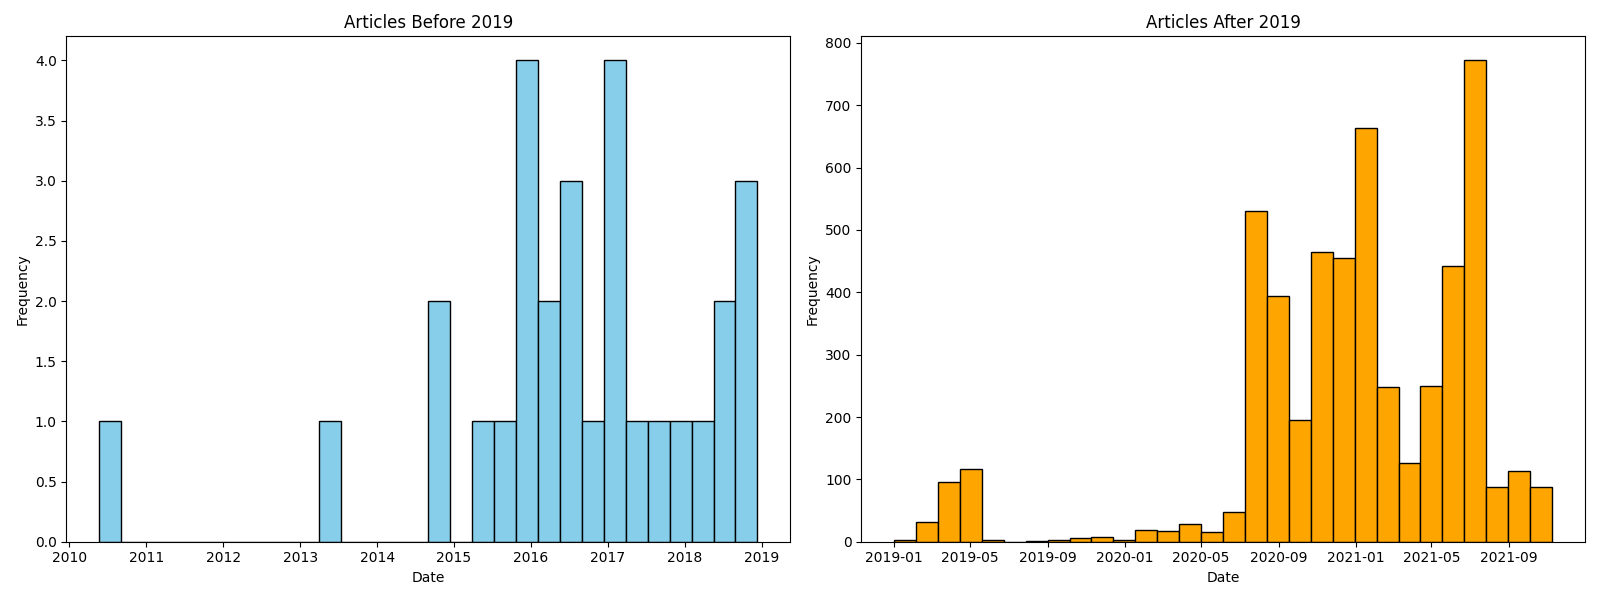
\includegraphics[width=0.9\linewidth]{figures/dates_hist.png}
    \caption{Articles published date distribution.}
    \label{fig:dates_hist}
\end{figure}

Most articles in the BAT dataset were written and published within the last six years, with only thirty-one articles published before 2019 (Figure \ref{fig:dates_hist}). Looking at these articles individually, they generally cover similar topics to those published after 2019 and therefore should not exhibit consequential differences in behaviour and characteristics.

\begin{figure}[htbp]
    \centering
    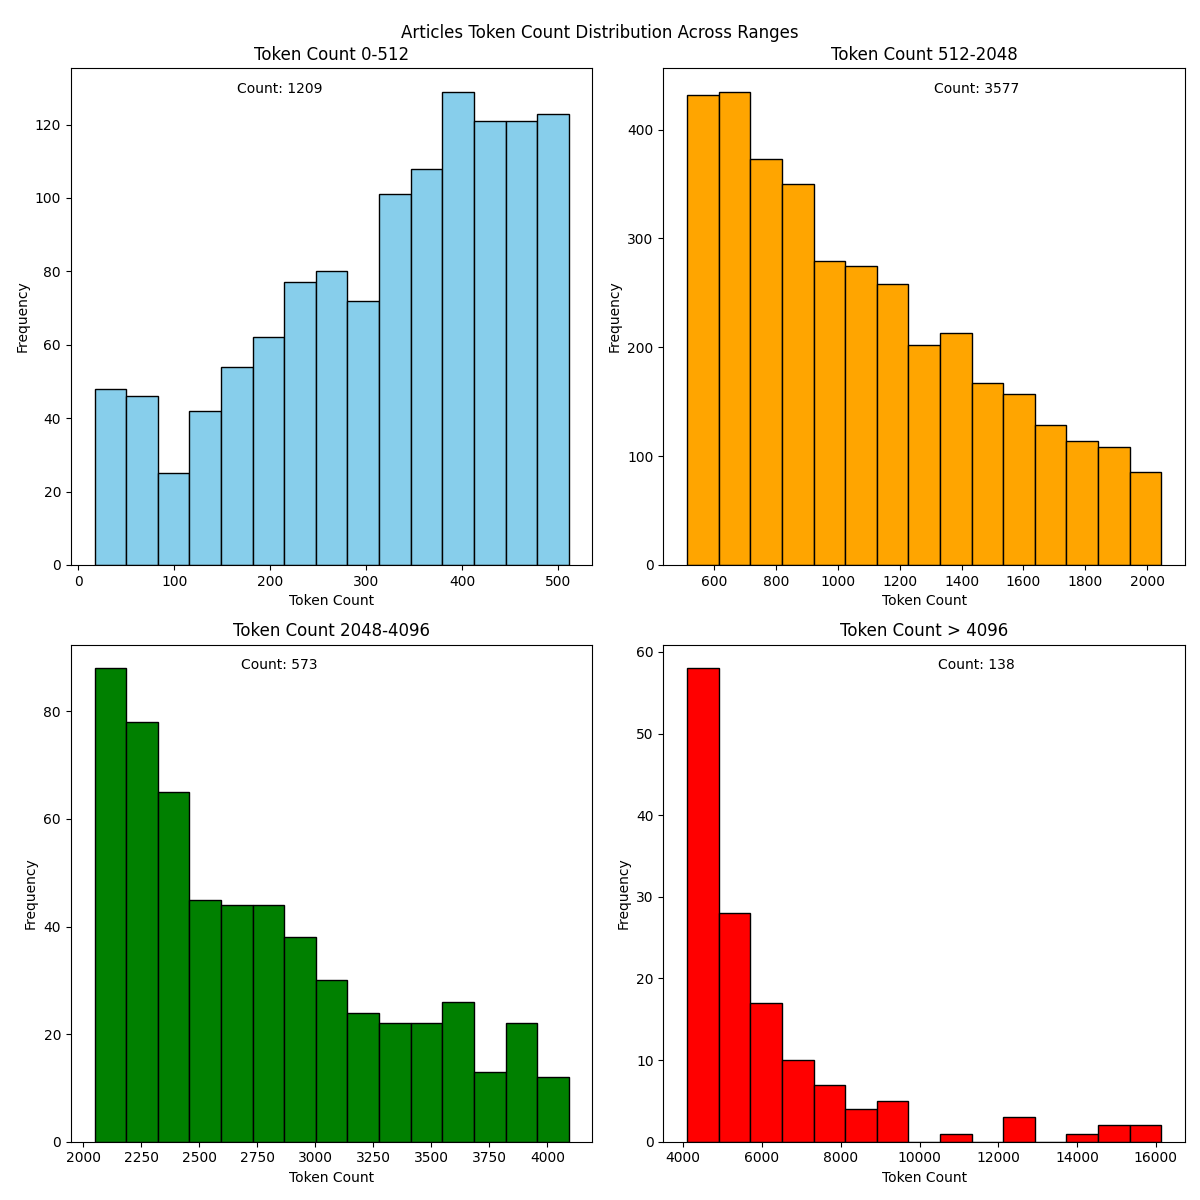
\includegraphics[width=0.8\linewidth]{figures/token_count_vx_split_hist.png}
    \caption{Articles tokens count distribution}
    \label{fig:token_hist_split}
\end{figure}

Analysis of articles token count can be seen in Figure \ref{fig:token_hist_split}. Note that sub-words are used as tokens in this analysis rather than whole words. The length of article content tokens ranges from 17 to 16,139, with an average length of 1,207.07 and a median value of 908 tokens. More than half of articles in the dataset have between 512 and 2,048 tokens. Only nine articles have more than 10,000 tokens, while 106 articles have fewer than 100 tokens. Furthermore, 1,209 articles contain 512 tokens or fewer, which is the maximum input length for BERT. Thus, when using BERT in its standard configuration, significant information loss is to be expected due to the token limit.

\begin{figure}[htbp]
    \centering
    \begin{subfigure}{0.49\linewidth}
        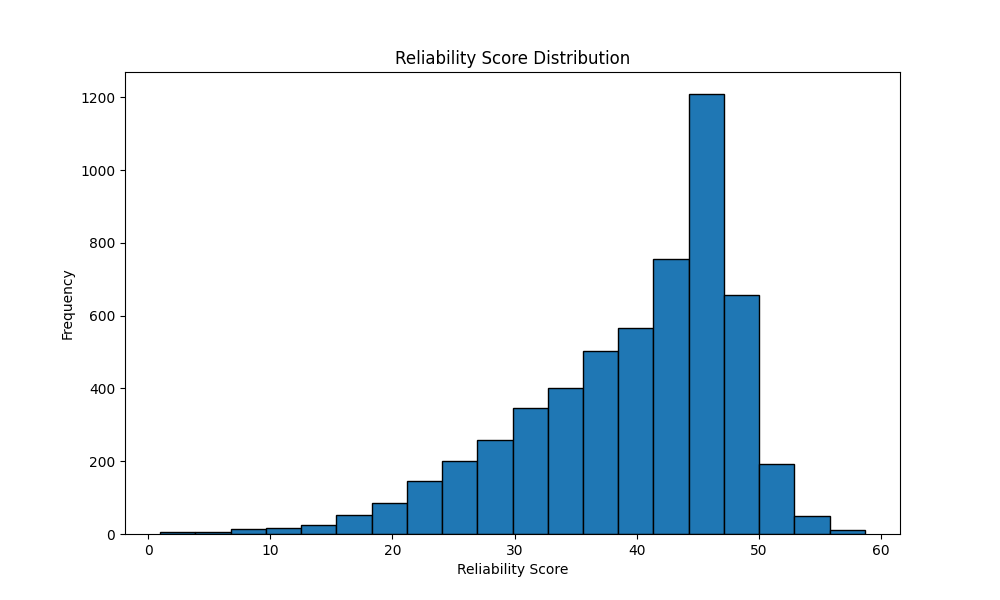
\includegraphics[width=1\linewidth]{figures/reliability_score_hist.png}
        \caption{Reliability score distribution.}
        \label{fig:reliability_score_hist}
    \end{subfigure}
    \begin{subfigure}{0.49\linewidth}
        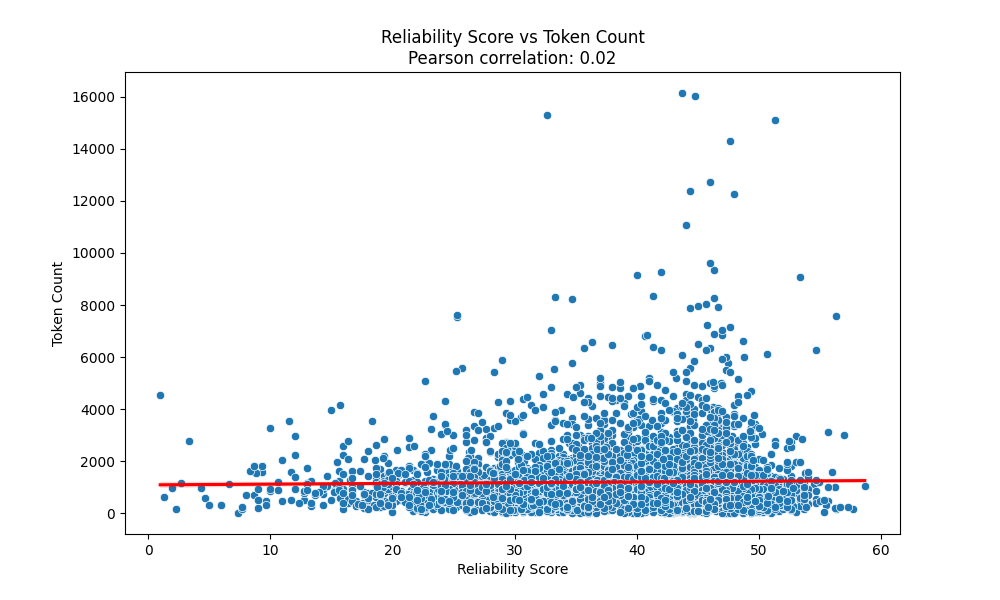
\includegraphics[width=1\linewidth]{figures/correlation_token_reliability_score.png}
        \caption{Pearson correlation.}
        \label{fig:pearson}
    \end{subfigure}
    \begin{subfigure}{0.56\linewidth}
        \centering
        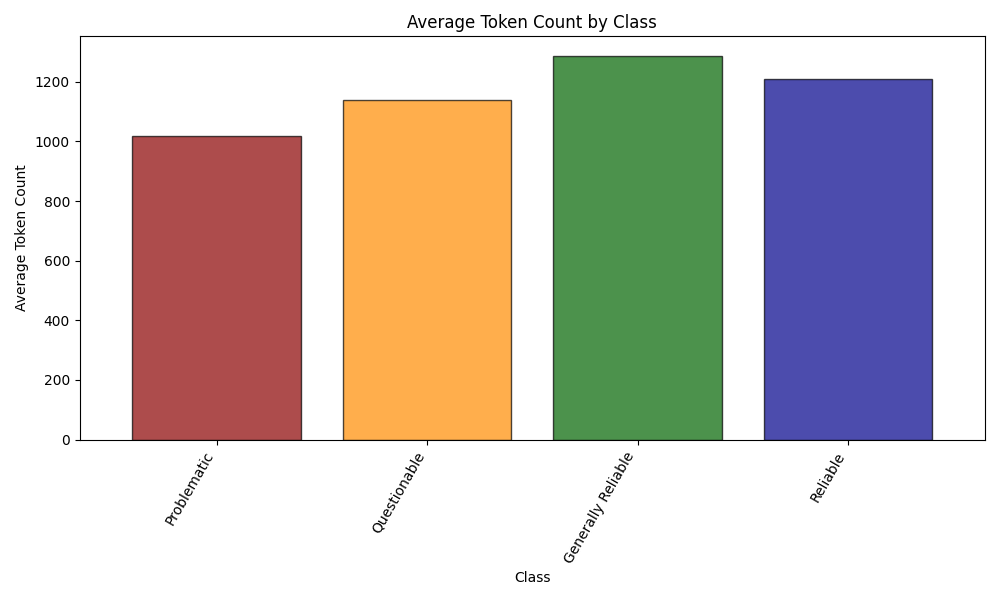
\includegraphics[width=1\linewidth]{figures/token_count_vx_per_class_hist.png}
        \caption{Average token count per class.}
        \label{fig:avg_token_per_class}
    \end{subfigure}
    \caption{Reliability score and token count analysis.}
    \label{fig:reliability_token_analysis}
\end{figure}

The articles reliability scores range from 1.0 to 58.67, with the majority scoring between 40 and 50. No articles  exceed a score of 60, despite the highest possible score being 64. Thus, only several hundreds of articles are rated low. The full histogram of the reliability scores is shown in Figure \ref{fig:reliability_score_hist}.

Figure \ref{fig:avg_token_per_class} also shows that all classes have similar average token count, close to the overall average. The 'Problematic' and 'Questionable' classes, being the two most biased, have lower average token count than the other two classes. However, further analysis (Figure \ref{fig:pearson}) reveals that there is virtually no linear relationship between token count and reliability score, with a Pearson correlation coefficient of 0.02. This indicates that the length of an article has no significant impact on its reliability score. In other words, longer articles are not necessarily more or less reliable than shorter ones based on the provided data.


%%% Local Variables: 
%%% mode: latex
%%% TeX-master: "thesis"
%%% End: 
\chapter{Dataset Building}
\label{cha:4}

\section{BAT dataset}

\subsection{Characteristics} \label{bat-characteristics}

The BAT dataset \cite{spinde-2023-bat} is chosen instead of NLPCSS \cite{chen-2020-nlpcss} for this project due to its article-level suitability and labels fluidity, as well additional metadata as it contains outlets information. It contains 6345 rows of manually labeled news articles from 255 English-speaking news outlets (US-based), originally scraped from Ad Fontes Media's website along with their respective \textbf{political bias} and \textbf{reliability scores}. Articles in the dataset encompassed a wide range of topics such as COVID-19, politics, and lifestyle. The political bias score measures the extent of political influence, ranging from -42 (most extreme left) to +42 (most extreme right). The reliability score reflects the article's truthfulness, with values ranging from 0 (least reliable, containing inaccurate or fabricated information) to 64 (most reliable, original fact reporting).

Both political bias and reliability scores on each article were rated using defined metrics and multiple sub-factors, performed by three randomly selected analysts from Ad Fontes Media's team of over 60 experts. The corresponding three scores were then averaged, producing the final article scores. Moreover, each group consists of analysts with different beliefs in the political spectrum i.e., left, center, and right.

The reliability score evaluates original fact reporting to analysis, opinion, propaganda, and inaccurate/fabricated information, with scores above 40 generally considered good and scores below 24 typically seen as problematic, scores between 24 and 40 suggest a variety of factors, including a strong presence of opinion and analysis or significant variability in reliability across different articles \cite{adfontes}. This metric is chosen as the main label in this project due to its correlation with textual-level bias: phrasing bias, spin bias, and statement bias described in Section \ref{media-bias-definition}

\begin{table}[htbp]
    \centering
    \begin{minipage}{0.9\linewidth}
        \begin{center}
            \small{Trump Win Validated by Quantum Blockchain System Recount of Votes}
        \end{center}
        \scriptsize{
            A recount of voting ballots nationwide was being done by elite units of the National Guard by early Sun. morning 8 Nov. To prevent fraud official ballots had been printed with an invisible, unbreakable code watermark and registered on a Quantum Blockchain System. As of this writing, in five states 14 million ballots had been put through a laser scanner – 78\% of which failed because there was no watermark to verify the ballot. Of those that failed 100\% had checked for Biden. An initial test showed that according to water marks on validated ballots fed into the Quantum Computer, Trump won re-election by over 80\% of the legal ballot cast. The final validated vote tallied in that test: Trump 73.5 million votes to Biden’s 25.9 million – and that didn’t even account for Trump votes that people observed being tossed and never accounted for. Interesting enough, those figures corresponded with the two men’s Twitter accounts: Trump had 88.8 million followers to Biden’s 16.6 million. Using ‘infrared’ equipment that read which ballots were real, or fake the elite National Guardsmen had been deployed to the twelve targeted states of Alabama, Arizona, Pennsylvania, Colorado, Texas, Wisconsin, Tennessee, Washington, Virginia, Delaware, Illinois and Kentucky. In all nationwide, over 500 National Guardsmen were on guard over all ballot counting units. There was much more to the tests for fraudulent voting. In addition to the watermark these official ballots also contained ink made of corn, which created an electronic radiation circuit ID that could trace the location of that ballot through GPS transmission. In other words, they could trace if the ballot was filled out by the person named on the ballot. The Trump team would be filing a number of lawsuits onThey had been preparing for this for a long time under an election fraud investigation called Project Veritas. Judicial Watch:“Our new study shows 1.8M excess, or ‘ghost’ voters in 353 counties across 29 states. The data highlights the recklessness of mailing blindly ballots/ballot applications to voter registration lists,”@TomFitton Watch more: at http://judicialwatch.org Pennsylvania alone Trump’s legal counsel Rudy Guliani had testimony of 50-60 poll watchers who claimed being deprived of an ability to inspect mail in ballots. Nationally, noted attorney Sydney Powell (rumored to be appointed the next FBI director) said, “Hammer and Scorecard – the NSA Security Software turned illegal Election Software – ran an algorithm that gave Biden a 3\% vote advantage in Wisconsin, Michigan, Pennsylvania, Georgia, Nevada and Arizona.”Rest assured, all legal issues would be accounted for by the time the Electoral College met on. By then real election results – post court battles – would determine all legally cast ballots. The joint session of Congress would make the election official on 3 Jan. 2021.}
    \end{minipage}
    \caption{Example of a biased article, reliability score: 4.67}
    \label{table:example-biased-article-1}
\end{table}

An example of a low-rated article can be seen in Table \ref{table:example-biased-article-1}. The deceptive article contains many wrongful claims and blatantly false events that did not happen in real life. In contrast, Table \ref{table:example-nonbiased-article-1} shows an example of a high-rated article. The content reports only facts regarding the event and statements from people related to the incident. Journalist opinions or political innuendos are non-existent.


\begin{table}[htbp]
    \centering
    \begin{minipage}{0.9\linewidth}
        \begin{center}
            \small{Trenton police officer takes own life in Plainsboro parking lot, officials say}
        \end{center}
        \scriptsize{
            A veteran Trenton police officer took his own life in a parking lot Wednesday, officials said. Sgt. Daniel Pagnotta, a 21-year-veteran of the department, died this morning in Plainsboro, according to a city spokesman.“Beloved by everyone in the Trenton Police Department, he was devoted to Trenton and police work,” Mayor Reed Gusciora said in a statement. The statement described Pagnotta as a devoted husband and father of two who loved soccer and making people laugh. His father, also named Dan, is a retired Trenton police officer.“Dan was proud to continue a legacy of law enforcement in his family,” Gusciora said. “Dan and his family are on our minds and in our hearts. He will be dearly missed.”}
    \end{minipage}
    \caption{Example of a non-biased article, reliability score: 57.67}
    \label{table:example-nonbiased-article-1}
\end{table}

\subsection{Extension}

The original BAT dataset only contains news titles and links (along with other metadata) and is missing the body content of articles. To overcome this, a Python script is written and executed, iteratively visiting each of the URLs from the dataset and scraping the news content. This was not an easy task as each website has its own unique structures and formats. Furthermore, the scraped text contains noises that are almost impossible to remove through the script. Some outlets such as The Nation, Chicago Tribune, and Truthout required manual intervention as the scraped text was duplicated over themselves. The current extended dataset contains 5270 rows of articles, mainly due to unavailable websites and missing articles.

To remove noises from article content, the text are then pre-processed extensively. All the content of every article in the dataset were joined into one single list, split into words, and then compared against an English word list \cite{dwyl-english-words}, resulting in a list of faulty words sorted by their occurences. Using this list, noisy patterns were analysed and handled through a combination of string and regex methods, and conjoined words were identified and fixed through a giant Python dictionary. This process is repeated more than several times until the contents are valuable enough to work with. Note that at this point some noises still remain within the text as it will take an extensive amount of time and manual labour to completely clean the text.

\begin{comment}
Explain further on preprocessing scraped text. More details on the preprocessing scripts?
\end{comment}

\subsection{Analysis}

\begin{figure}[htbp]
    \centering
    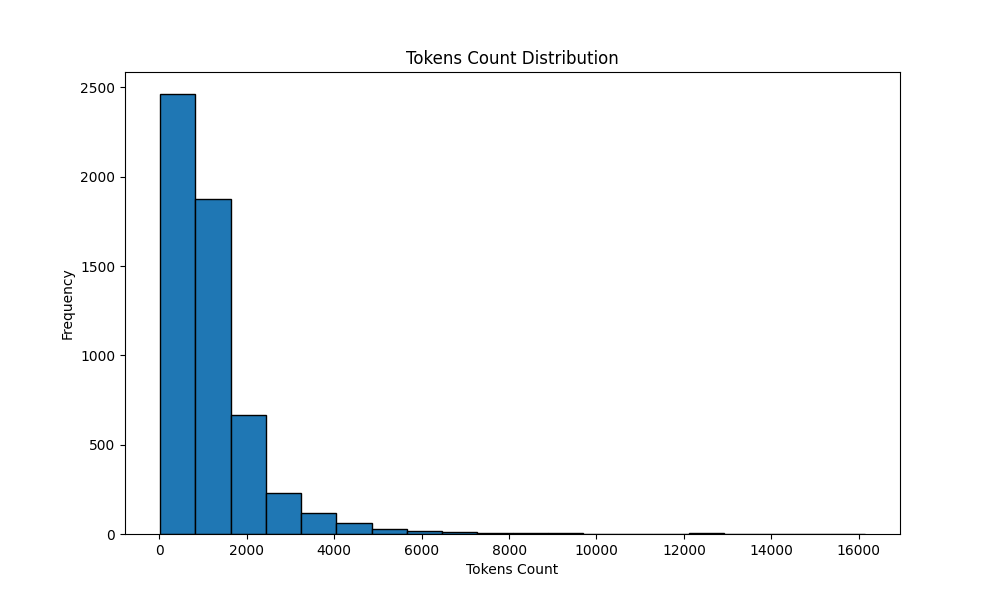
\includegraphics[width=0.9\linewidth]{figures/tokens_count_vx_hist.png}
    \caption{Articles token count distribution}
    \label{fig:tokens_hist}
\end{figure}

\begin{figure}[htbp]
    \centering
    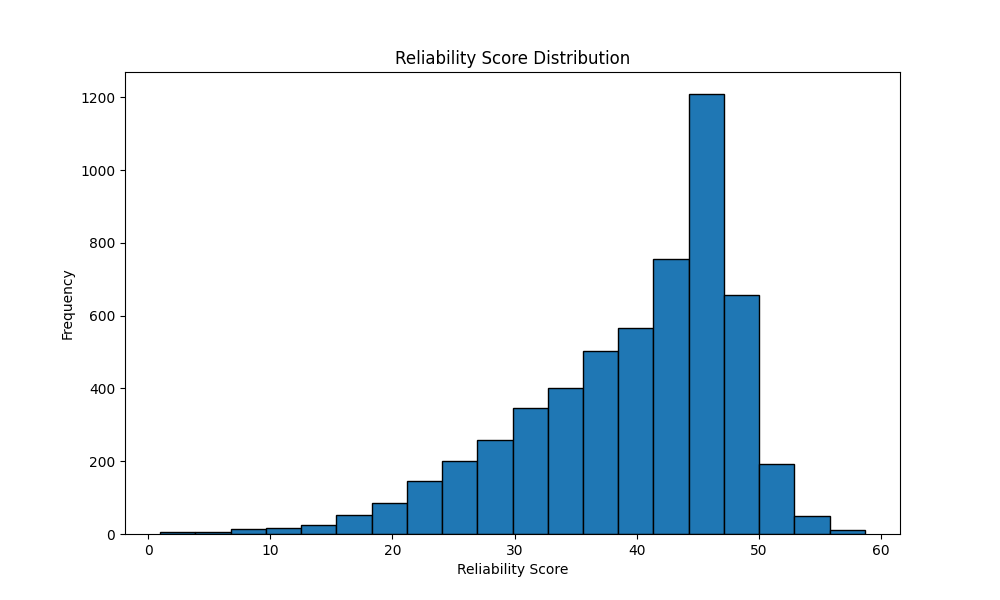
\includegraphics[width=0.9\linewidth]{figures/reliability_score_hist.png}
    \caption{Reliability score distribution}
    \label{fig:reliability_score_hist}
\end{figure}

The article content tokens length ranges between 22 tokens to 15530 tokens, with an average length of 1186.5 and a median value of 887 tokens. Only 9 articles have more than 10000 tokens, while there are 106 of articles with less than 100 tokens. Furthermore, only 1193 articles stay between 512 tokens, which is the limit for BERT input. The articles reliability score ranges from 1.0 to 58.67, the majority have a value between 20 - 50. Not a single articles were rated more than 60 despite the highest score being 64. Visualisations can be seen in both Figure \ref{fig:tokens_hist} and Figure \ref{fig:reliability_score_hist}, as well as Figure \ref{fig:tokens_hist_split}


\begin{figure}[htbp]
    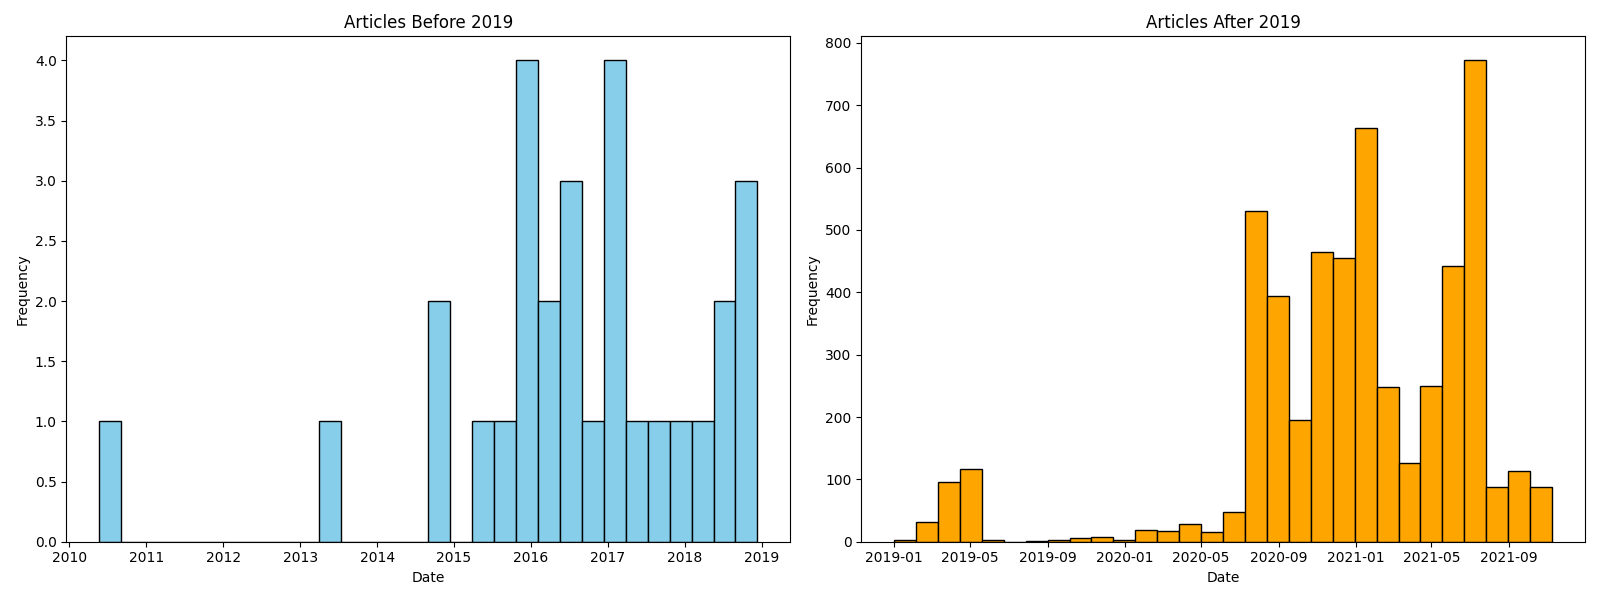
\includegraphics[width=0.9\linewidth]{figures/dates_hist.png}
    \caption{Article dates distribution}
    \label{fig:dates_hist}
\end{figure}

Most articles are written and published within the last 6 years, with only 29 articles, a minuscule percentage, published before 2019, shown in Figure \ref{fig:dates_hist}. From my personal analysis, these 29 articles generally contain similar topics to articles published after 2019 and therefore should not hold any difference in behaviour and characteristics.


\begin{figure}[htbp]
    \centering
    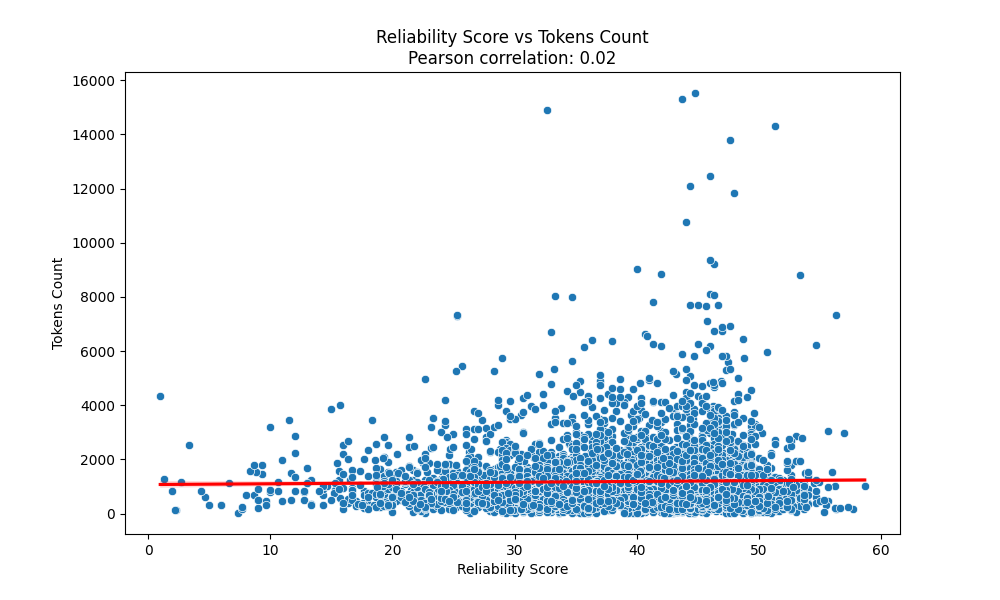
\includegraphics[width=0.9\linewidth]{figures/correlation_tokens_reliability_score.png}
    \caption{Pearson correlation between token count and reliability score}
    \label{fig:pearson_correlation}
\end{figure}


Figure \ref{fig:avg_tokens_count_per_class} shows that all classes seem to have similar token count, close to the overall average. Class 'Problematic' and 'Questionable', being the two most biased classes, seem to have lower average token count than the two other classes. However, further analysis (Figure \ref{fig:pearson_correlation}) shows that there is virtually no linear relationship between token count and reliability score, with a Pearson correlation coefficient is 0.02. This proves that the length of an article has no significant impact on its reliability score. In other words, longer articles are not necessarily more or less reliable than shorter ones based on the provided data.

\begin{comment}
relationship between words and reliability score?
\end{comment}


% \section{Conclusion}
% The final section of the chapter gives an overview of the important results
% of this chapter. This implies that the introductory chapter and the
% concluding chapter don't need a conclusion.


%%% Local Variables: 
%%% mode: latex
%%% TeX-master: "thesis"
%%% End: 

\chapter{Evaluation}
\label{cha:5}


For every method, precision, recall, and F1 score is evaluated on both overall and per class performance.

\begin{table}[htbp]
    \centering
    \footnotesize
    \begin{tabular}{| c | c | c | c | c |}
        \hline                            \textbf{Method}  & \textbf{Class}     & \textbf{Precision} & \textbf{Recall} & \textbf{F1}     \\\cline{1-5}
        \multirow{5}{*}{BoW + LR}                          & Problematic        & 0.38               & 0.41            & 0.39            \\
                                                           & Questionable       & 0.34               & 0.31            & 0.33            \\
                                                           & Generally Reliable & 0.36               & 0.40            & 0.38            \\
                                                           & Reliable           & 0.85               & 0.83            & 0.84            \\\cline{2-5}
                                                           & Overall            & 0.6922             & 0.6818          & 0.6865          \\
        \hline
        \multirow{5}{*}{TF-IDF + LR}                       & Problematic        & 1.00               & 0.11            & 0.20            \\
                                                           & Questionable       & 0.47               & 0.17            & 0.25            \\
                                                           & Generally Reliable & 0.36               & 0.31            & 0.33            \\
                                                           & Reliable           & 0.79               & 0.94            & 0.86            \\\cline{2-5}
                                                           & Overall            & 0.6904             & 0.7117          & 0.6725          \\
        \hline
        \multirow{5}{*}{BoW + MLP}                         & Problematic        & 0.38               & 0.44            & 0.41            \\
                                                           & Questionable       & 0.33               & 0.35            & 0.34            \\
                                                           & Generally Reliable & 0.41               & 0.42            & 0.42            \\
                                                           & Reliable           & 0.88               & 0.85            & 0.86            \\\cline{2-5}
                                                           & Overall            & 0.7162             & 0.7065          & 0.7110          \\
        \hline
        \multirow{5}{*}{BERT FT}                           & Problematic        & 0.43               & 0.44            & 0.44            \\
                                                           & Questionable       & 0.29               & 0.39            & 0.33            \\
                                                           & Generally Reliable & 0.44               & 0.48            & 0.46            \\
                                                           & Reliable           & 0.90               & 0.83            & 0.86            \\\cline{2-5}
                                                           & Overall            & 0.7359             & 0.7065          & 0.7193          \\
        \hline
        \multirow{5}{*}{Longformer FT}                     & Problematic        & 0.48               & 0.48            & 0.48            \\
                                                           & Questionable       & 0.44               & 0.50            & 0.47            \\
                                                           & Generally Reliable & 0.47               & 0.59            & 0.52            \\
                                                           & Reliable           & 0.92               & 0.84            & 0.88            \\\cline{2-5}
                                                           & Overall            & 0.7708             & 0.7434          & 0.7544          \\
        \hline
        \multirow{5}{*}{Bigbird FT}                        & Problematic        & 0.38               & 0.41            & 0.39            \\
                                                           & Questionable       & 0.32               & 0.46            & 0.38            \\
                                                           & Generally Reliable & 0.40               & 0.47            & 0.43            \\
                                                           & Reliable           & 0.91               & 0.81            & 0.86            \\\cline{2-5}
                                                           & Overall            & 0.7377             & 0.6959          & 0.7131          \\
        \hline
        \multirow{5}{*}{BERT C-FT}                         & Problematic        & 0.45               & 0.48            & 0.46            \\
                                                           & Questionable       & 0.39               & 0.52            & 0.45            \\
                                                           & Generally Reliable & 0.42               & 0.50            & 0.46            \\
                                                           & Reliable           & 0.91               & 0.81            & 0.86            \\\cline{2-5}
                                                           & Overall            & 0.7472             & 0.7112          & 0.7257          \\
        \hline
        % \multirow{5}{*}{Hierarchical BERT, CLS-Pooling}    & Problematic        & 0.44               & 0.67            & 0.53            \\
        %                                                    & Questionable       & 0.41               & 0.48            & 0.44            \\
        %                                                    & Generally Reliable & 0.39               & 0.50            & 0.44            \\
        %                                                    & Reliable           & 0.91               & 0.79            & 0.84            \\\cline{2-5}
        %                                                    & Overall            & 0.7440             & 0.6994          & 0.7163          \\
        % \hline
        % \multirow{5}{*}{Hierarchical MAGPIE, CLS-Pooling}  & Problematic        & 0.46               & 0.63            & 0.53            \\
        %                                                    & Questionable       & 0.36               & 0.41            & 0.38            \\
        %                                                    & Generally Reliable & 0.41               & 0.55            & 0.47            \\
        %                                                    & Reliable           & 0.93               & 0.80            & 0.86            \\\cline{2-5}
        %                                                    & Overall            & 0.7577             & 0.7117          & 0.7293          \\
        % \hline
        \multirow{5}{*}{Hierarchical MAGPIE, Mean-Pooling} & Problematic        & 0.50               & 0.63            & 0.56            \\
                                                           & Questionable       & 0.46               & 0.50            & 0.48            \\
                                                           & Generally Reliable & 0.47               & 0.59            & 0.52            \\
                                                           & Reliable           & 0.92               & 0.83            & 0.87            \\\cline{2-5}
                                                           & Overall            & \textbf{0.7743}    & \textbf{0.7434} & \textbf{0.7554} \\
        \hline
    \end{tabular}
    \caption{Evaluation table, with title and content of articles as features}
    \label{table:eval}
\end{table}

Table \ref{table:eval} shows the evaluation of all methods given only title and content of articles as features. It can be seen that frequency-based approaches such as BoW and TF-IDF performed generally decent. However, looking at per-class metrics, it is evident that the overall scores are heavily influenced by the performance of the 'Reliable' class due to its large support. On all of the other less represented classes, the models' performance suffered with much lower F1 scores with the TF-IDF + LR model having the worst F1 score on the 'Problematic' class. The BoW + MLP model achieved slight improvement in almost all instances compared to its predecessor due to the use of neural network. A typical BERT fine-tuning outperformed all frequency-based methods, though only with a close margin compared to the BoW + MLP model. The BERT sliding window fine-tuning (BERT SW FT) method outperformed all BoW and TF-IDF methods, also performing slightly better to a standard BERT fine-tuning of the first 512 tokens. Similarly, the CLS methods mostly outperformed traditional methods with best F1 score on the 'Problematic' class, able to generalise on the most biased class. While BERT CLS achieved slightly worse performance compared to the two fine-tuning methods, \textbf{MAGPIE CLS performed best among all other methods with the highest overall precision, recall, and F1 score.}

\begin{table}[htbp]
    \centering
    \footnotesize
    \begin{tabular}{| c | c | c | c | c |}
        \hline                            \textbf{Method}  & \textbf{Class}     & \textbf{Precision} & \textbf{Recall} & \textbf{F1}     \\\cline{1-5}
        \multirow{5}{*}{Outlet majority}                   & Problematic        & 0.56               & 0.70            & 0.62            \\
                                                           & Questionable       & 0.58               & 0.46            & 0.52            \\
                                                           & Generally Reliable & 0.56               & 0.53            & 0.54            \\
                                                           & Reliable           & 0.91               & 0.93            & 0.92            \\\cline{2-5}
                                                           & Overall            & 0.7945             & \textbf{0.7996} & \textbf{0.7959} \\
        \hline
        \multirow{5}{*}{BERT FT}                           & Problematic        & 0.65               & 0.56            & 0.60            \\
                                                           & Questionable       & 0.45               & 0.50            & 0.47            \\
                                                           & Generally Reliable & 0.44               & 0.62            & 0.52            \\
                                                           & Reliable           & 0.94               & 0.84            & 0.88            \\\cline{2-5}
                                                           & Overall            & \textbf{0.8186}    & 0.7883          & 0.7504          \\
        \hline
        \multirow{5}{*}{Longformer FT}                     & Problematic        & 0.60               & 0.44            & 0.51            \\
                                                           & Questionable       & 0.45               & 0.56            & 0.50            \\
                                                           & Generally Reliable & 0.44               & 0.53            & 0.48            \\
                                                           & Reliable           & 0.91               & 0.85            & 0.88            \\\cline{2-5}
                                                           & Overall            & 0.7676             & 0.7434          & 0.7529          \\
        \hline
        \multirow{5}{*}{Bigbird FT}                        & Problematic        & 0.41               & 0.44            & 0.43            \\
                                                           & Questionable       & 0.39               & 0.52            & 0.45            \\
                                                           & Generally Reliable & 0.43               & 0.53            & 0.48            \\
                                                           & Reliable           & 0.92               & 0.82            & 0.86            \\\cline{2-5}
                                                           & Overall            & 0.7538             & 0.7170          & 0.7318          \\
        \hline
        \multirow{5}{*}{BERT C-FT}                         & Problematic        & 0.46               & 0.41            & 0.43            \\
                                                           & Questionable       & 0.41               & 0.48            & 0.44            \\
                                                           & Generally Reliable & 0.46               & 0.56            & 0.51            \\
                                                           & Reliable           & 0.91               & 0.84            & 0.87            \\\cline{2-5}
                                                           & Overall            & 0.7585             & 0.7359          & 0.7451          \\
        \hline
        % \multirow{5}{*}{Hierarchical BERT, CLS-Pooling}   & Problematic        & 0.37               & 0.59            & 0.46            \\
        %                                                   & Questionable       & 0.32               & 0.43            & 0.37            \\
        %                                                   & Generally Reliable & 0.40               & 0.47            & 0.43            \\
        %                                                   & Reliable           & 0.92               & 0.79            & 0.85            \\\cline{2-5}
        %                                                   & Overall            & 0.7384             & 0.6871          & 0.7071          \\
        % \hline
        % \multirow{5}{*}{Hierarchical MAGPIE, CLS-Pooling} & Problematic        & 0.42               & 0.52            & 0.47            \\
        %                                                   & Questionable       & 0.35               & 0.43            & 0.38            \\
        %                                                   & Generally Reliable & 0.43               & 0.55            & 0.48            \\
        %                                                   & Reliable           & 0.93               & 0.82            & 0.87            \\\cline{2-5}
        %                                                   & Overall            & 0.76034            & 0.7170          & 0.7342          \\
        % \hline
        \multirow{5}{*}{Hierarchical MAGPIE, Mean-Pooling} & Problematic        & 0.42               & 0.59            & 0.49            \\
                                                           & Questionable       & 0.35               & 0.41            & 0.38            \\
                                                           & Generally Reliable & 0.42               & 0.56            & 0.48            \\
                                                           & Reliable           & 0.93               & 0.80            & 0.86            \\\cline{2-5}
                                                           & Overall            & 0.7591             & 0.7117          & 0.7298          \\
        \hline
    \end{tabular}
    \caption{Evaluation table, with outlet information as additional features (outlet + title + content)}
    \label{table:eval-outlet}
\end{table}

Table \ref{table:eval-outlet} shows the evaluation of methods, given the article's outlet information as additional features to the title and content. As a comparison, \textbf{using outlet information as the sole feature without any other information (with majority votes) outperformed all methods on overall recall and F1 scores}. This result signified how influential outlet information can be in terms of classifying media bias, with regards to this specific dataset and circumstances. Out of all the other methods, BERT fine-tuning reigned superior with the best overall precision score and a particularly strong F1 score on the 'Problematic' class, performing slightly better than the sliding window implementation (BERT SW FT). Interestingly, both BERT CLS and MAGPIE CLS methods were not able to capitalise on the outlet information as well as BERT FT and BERT SW FT as both CLS methods only saw little improvement compared to when outlet features were unavailable.

All methods demonstrate reasonably well with overall precision, recall, and F1 scores above 0.67, with a particularly strong performance on the 'Reliable' class, achieving F1 scores consistently above 0.84.


%%% Local Variables: 
%%% mode: latex
%%% TeX-master: "thesis"
%%% End: 

\chapter{Evaluation}
\label{cha:6}

All methods are implemented using the PyTorch \cite{paszke-2017-pytorch} and transformer \cite{wolf-2020-huggingface} package from HuggingFace. BERT model used is 'bert-base-cased'. The batch size is set to 8, with epochs ranging between 3-5. Learning rate is set to either 1e-5 and 2e-5, with a linear warmup steps of 162 (10\% of total training steps). For every method, precision, recall, and F1 score is evaluated on both overall and per class performance. It is particularly important to assess how well the model classify biased articles. Chunk size is 512 for chunk-based methods.

\begin{table}[htbp]
    \centering
    \small
    \begin{tabular}{| c | c | c | c | c |}
        \hline                            Method & Class              & Precision & Recall & F1     \\\cline{1-5}
        \multirow{5}{*}{BoW + LR}                & Problematic        & 0.38      & 0.41   & 0.39   \\
                                                 & Questionable       & 0.34      & 0.31   & 0.33   \\
                                                 & Generally Reliable & 0.36      & 0.40   & 0.38   \\
                                                 & Reliable           & 0.85      & 0.83   & 0.84   \\
                                                 & Overall            & 0.6922    & 0.6818 & 0.6865 \\
        \hline
        \multirow{5}{*}{TF-IDF + LR}             & Problematic        & 1.00      & 0.11   & 0.20   \\
                                                 & Questionable       & 0.47      & 0.17   & 0.25   \\
                                                 & Generally Reliable & 0.36      & 0.31   & 0.33   \\
                                                 & Reliable           & 0.79      & 0.94   & 0.86   \\
                                                 & Overall            & 0.6904    & 0.7117 & 0.6725 \\
        \hline
        \multirow{5}{*}{Outlet majority}         & Problematic        & 0.56      & 0.70   & 0.62   \\
                                                 & Questionable       & 0.58      & 0.46   & 0.52   \\
                                                 & Generally Reliable & 0.56      & 0.53   & 0.54   \\
                                                 & Reliable           & 0.91      & 0.93   & 0.92   \\
                                                 & Overall            & 0.7945    & 0.7996 & 0.7959 \\
        \hline
        \multirow{5}{*}{BERT FT}                 & Problematic        & 0.43      & 0.44   & 0.44   \\
                                                 & Questionable       & 0.29      & 0.39   & 0.33   \\
                                                 & Generally Reliable & 0.44      & 0.48   & 0.46   \\
                                                 & Reliable           & 0.90      & 0.83   & 0.86   \\
                                                 & Overall            & 0.7359    & 0.7065 & 0.7193 \\
        \hline
        \multirow{5}{*}{BERT SW FT}              & Problematic        & 0.45      & 0.48   & 0.46   \\
                                                 & Questionable       & 0.39      & 0.52   & 0.45   \\
                                                 & Generally Reliable & 0.42      & 0.50   & 0.46   \\
                                                 & Reliable           & 0.91      & 0.81   & 0.86   \\
                                                 & Overall            & 0.7472    & 0.7112 & 0.7257 \\
        \hline
        \multirow{5}{*}{BERT CLS}                & Problematic        & 0.44      & 0.67   & 0.53   \\
                                                 & Questionable       & 0.41      & 0.48   & 0.44   \\
                                                 & Generally Reliable & 0.39      & 0.50   & 0.44   \\
                                                 & Reliable           & 0.91      & 0.79   & 0.84   \\
                                                 & Overall            & 0.7440    & 0.6994 & 0.7163 \\
        \hline
        \multirow{5}{*}{MAGPIE CLS}              & Problematic        & 0.46      & 0.63   & 0.53   \\
                                                 & Questionable       & 0.36      & 0.41   & 0.38   \\
                                                 & Generally Reliable & 0.41      & 0.55   & 0.47   \\
                                                 & Reliable           & 0.93      & 0.80   & 0.86   \\
                                                 & Overall            & 0.7577    & 0.7117 & 0.7293 \\
        \hline
    \end{tabular}
    \caption{Evaluation table, with features only including title and content of articles}
    \label{table:eval}
\end{table}



From Table \ref{table:eval} it can be seen that frequency-based approaches such as BoW and TF-IDF perform generally well. Including outlet information as features only slighty improve the performance. However, when we look at per-class metrics, it can be seen that the overall scores are heavily influenced by the performance of class 'Reliable' due to its large support. Evidently, the model suffers when classifying underrepresented classes. Furthermore, TF-IDF model seems to perform significantly worse in the 'Problematic' class.

Fine-tuning BERT only performed slightly better than BoW method. In this method 'bert-base-cased' is used instead of 'bert-base-uncased' to reserve differences in capitalised words, which can be crucial. Moreover, incorporating outlet information as features moderately increase the performance in all accounts.

As a comparison, using solely outlet information without any textual information (with majority votes) outperformed all baseline methods both overall and in every class. This result signifies how influential outlet information can be used to classify media bias.


The sliding window method outperformed both BoW and TF-IDF methods, while performing slightly better to a standard BERT fine-tuning of the first 512 tokens. However, with the outlet information included, BERT fine-tuning still reigned superior with a particularly strong f1 score on the "Problematic" class.

For the CLS method, two different language models are used: BERT and MAGPIE, to encode the input in a higher dimensional space. Both approaches with the CLS method are evaluated. A chunk size of 512 is used, 2 transformer layers, learning rate 1e-5, 162 warmup steps (10\% of training steps), 0.2 dropout probability, and 3 epochs.


Similarly, the CLS method mostly outperformed the baselines. However, with outlet information included the CLS methods performed somewhat worse, particularly on the most biased "Problematic" class. Compared to the sliding window, the MAGPIE CLS method performed slightly better while only using 2 transformer layer instead of 12 in the standard fine-tuning operation.


\begin{table}[htbp]
    \centering
    \small
    \begin{tabular}{| c | c | c | c | c |}
        \hline                            Method & Class              & Precision & Recall & F1     \\\cline{1-5}
        \multirow{5}{*}{Outlet majority}         & Problematic        & 0.56      & 0.70   & 0.62   \\
                                                 & Questionable       & 0.58      & 0.46   & 0.52   \\
                                                 & Generally Reliable & 0.56      & 0.53   & 0.54   \\
                                                 & Reliable           & 0.91      & 0.93   & 0.92   \\
                                                 & Overall            & 0.7945    & 0.7996 & 0.7959 \\
        \hline
        \multirow{5}{*}{BERT FT}                 & Problematic        & 0.65      & 0.56   & 0.60   \\
                                                 & Questionable       & 0.45      & 0.50   & 0.47   \\
                                                 & Generally Reliable & 0.44      & 0.62   & 0.52   \\
                                                 & Reliable           & 0.94      & 0.84   & 0.88   \\
                                                 & Overall            & 0.8186    & 0.7883 & 0.7504 \\
        \hline
        \multirow{5}{*}{BERT SW FT}              & Problematic        & 0.46      & 0.41   & 0.43   \\
                                                 & Questionable       & 0.41      & 0.48   & 0.44   \\
                                                 & Generally Reliable & 0.46      & 0.56   & 0.51   \\
                                                 & Reliable           & 0.91      & 0.84   & 0.87   \\
                                                 & Overall            & 0.7585    & 0.7359 & 0.7451 \\
        \hline
        \multirow{5}{*}{BERT CLS}                & Problematic        & 0.37      & 0.59   & 0.46   \\
                                                 & Questionable       & 0.32      & 0.43   & 0.37   \\
                                                 & Generally Reliable & 0.40      & 0.47   & 0.43   \\
                                                 & Reliable           & 0.92      & 0.79   & 0.85   \\
                                                 & Overall            & 0.7384    & 0.6871 & 0.7071 \\
        \hline
        \multirow{5}{*}{MAGPIE CLS}              & Problematic        & 0.42      & 0.52   & 0.47   \\
                                                 & Questionable       & 0.35      & 0.43   & 0.38   \\
                                                 & Generally Reliable & 0.43      & 0.55   & 0.48   \\
                                                 & Reliable           & 0.93      & 0.82   & 0.87   \\
                                                 & Overall            & 0.76034   & 0.7170 & 0.7342 \\
        \hline
    \end{tabular}
    \caption{Evaluation table, with outlet information as additional features (outlet + title + content)}
    \label{table:eval-outlet}
\end{table}


%%% Local Variables: 
%%% mode: latex
%%% TeX-master: "thesis"
%%% End: 


% If you have appendices:
\appendixpage*          % if wanted
\appendix
\chapter{The First Appendix}
\label{app:A}
Appendices hold useful data which is not essential to understand the work
done in the master's thesis. An example is a (program) source.
An appendix can also have sections as well as figures and references\cite{h2g2}.

\section{More Lorem}
\lipsum[50]

\subsection{Lorem 15--17}
\lipsum[15-17]

\subsection{Lorem 18--19}
\lipsum[18-19]

\section{Lorem 51}
\lipsum[51]

%%% Local Variables: 
%%% mode: latex
%%% TeX-master: "thesis"
%%% End: 

% ... and so on until
\chapter{The Last Appendix}
\label{app:n}
Appendices are numbered with letters, but the sections and subsections use
arabic numerals, as can be seen below.

\section{Lorem 20-24}
\lipsum[20-24]

\section{Lorem 25-27}
\lipsum[25-27]

%%% Local Variables: 
%%% mode: latex
%%% TeX-master: "thesis"
%%% End: 


\backmatter
% The bibliography comes after the appendices.
% You can replace the standard "abbrv" bibliography style by another one.
\bibliographystyle{abbrv}
\bibliography{references}

\end{document}

%%% Local Variables: 
%%% mode: latex
%%% TeX-master: t
%%% End: 
